%%%%%%%%%%%%%%%%%%%%%%%%%%%%%%%%%%%%%%%%%%%%%%%%%%%%%%%%%%%%%%%%%%%%%%%%%%%%%%%
%
% Purpose:  Validation part of V&V for the RadiationPressure model
%
%
%%%%%%%%%%%%%%%%%%%%%%%%%%%%%%%%%%%%%%%%%%%%%%%%%%%%%%%%%%%%%%%%%%%%%%%%%%%%%%%

\section{Validation}

%%% code imported from old template structure
%\test{<Title>}\label{test:<label>}
%\begin{description}
%\item[Purpose:] \ \newline
%<description>
%\item[Requirements:] \ \newline
%By passing this test, the universal time module
%partially satisfies requirement~\ref{reqt:<label1>} and
%completely satisfies requirement~\ref{reqt:<label2>}.
%\item[Procedure:]\ \newline
%<procedure>
%\item[Results:]\ \newline
%<results>
%\end{description}



\subsection{Validation of Flux-Vehicle Interaction-Model Principles}
\test{Flux-Vehicle Interaction Model Principles}
  \label{test:flux_vehicle_interaction}
  \begin{description}
    \item[Purpose:] \ \newline
      The purpose of this test is to validate that radiation-interaction
      can be modeled to reasonable accuracy by a combination of specular
      reflection, diffuse reflection, absorption, and emission.
    \item[Requirements:] \ \newline
      By passing this test, the model satisfies
      requirement~\ref{reqt:functional_interaction}.
    \item[Procedure:]\ \newline
      A number of test surfaces were run.
      Figure~\ref{fig:ivv_surface_profiles} shows the reflections
      for a series of four surfaces of progressively increasing roughness
      (and hence higher $\delta $, the weighting towards diffuse reflection).
      Each of these surfaces was tested with 3 different
      albedos, across a range of incident angles.  For each
      incident angle, 10\textsuperscript{6} ``photons'' were
      ``fired'' at the surface and the subsequent reflection or absorption
      recorded (see Figure \ref{fig:ivv_surface_profiles} for reflection
			characteristics).

      \begin{figure}[!ht]
        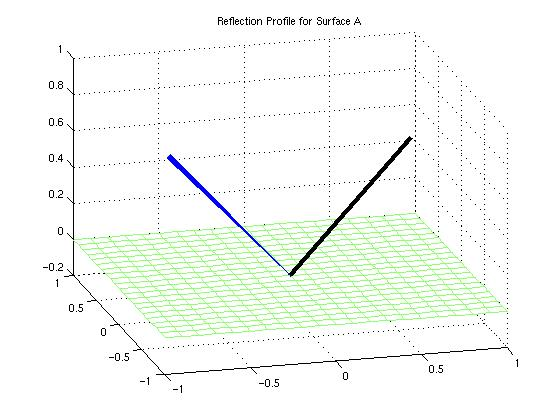
\includegraphics[width=95mm]{figs/sda/reflection1_sda.jpg}
        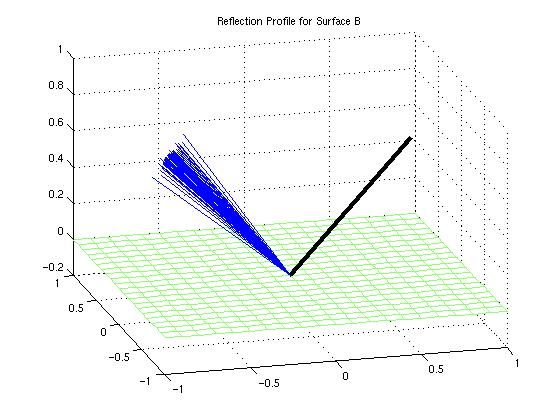
\includegraphics[width=95mm]{figs/sda/reflection2_sda.jpg}
        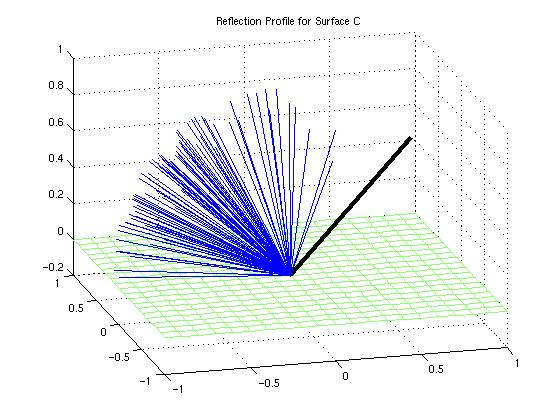
\includegraphics[width=95mm]{figs/sda/reflection3_sda.jpg}
        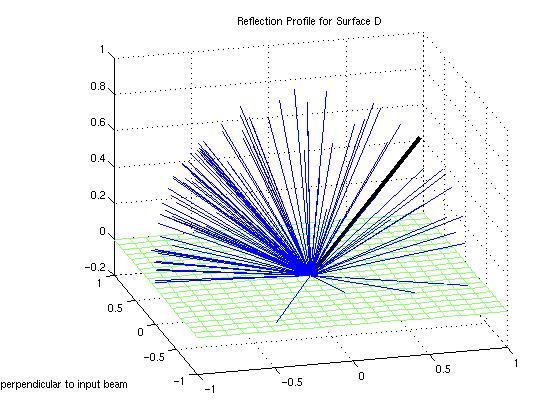
\includegraphics[width=95mm]{figs/sda/reflection4_sda.jpg}
        
\includegraphics[width=105mm,height=70mm]{figs/blank.jpg}
        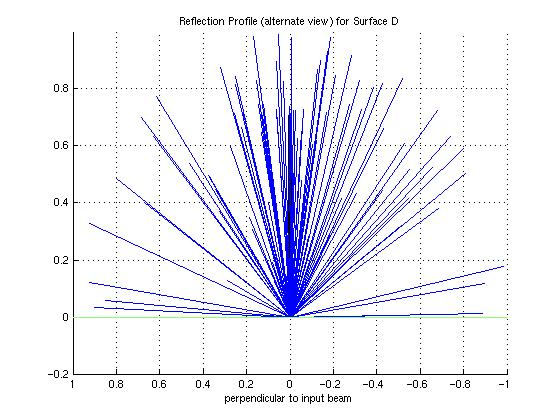
\includegraphics[width=75mm]{figs/sda/reflection5_sda.jpg}
        \caption{Reflection characteristics from four surfaces}
        \label{fig:ivv_surface_profiles}
      \end{figure}

      The vectors associated with photon reflections were averaged and
      compared to the theoretical average for thin-film
      interactions, equation \vref{eqn:s_hat_average}.

      \begin{equation*}
           \langle \hat{s}\rangle =\left[\begin{matrix}-0.5\;\sin \phi
           \;\left(1+e^{-\frac{1}{c}}\right)\\0\\\cos \phi
           \;e^{-\frac{1}{c}}\end{matrix}\right]
        \end{equation*}


      This theoretical value includes the possibility that a photon
      could be reflected downward as its terminal state, while the
      simulation took downward reflected photons and operated on them
      again until they were either absorbed by the surface, or
      reflected away from the surface.

 			In this representation, the x-axis is the negative of the projection
			of the incident radiation onto the surface;
			the z-axis is perpendicular to the surface, pointing outward
			the y-axis is parallel to the surface, and completes the right-hand
			coordinate system; \textit{c} represents the ``smoothness'' of the surface.

      The cumulative vector force calculated from the
      interactions of all photons for any given angle and surface was
      then compared with a best-fit bulk approximation that assigned some
      fraction of the incident photons to specular reflection, some to
      diffuse reflection, and some to absorption and subsequent
      emission.
    \clearpage

    \item[Results:]\ \newline
     The results section is divided into two parts: a comparison of the
     values for the unit-vector associated with reflection, and a
     comparison of the values for the force.

     \subsubsection{Unit-vector Comparisons}


      The average unit-reflection-vector, $\langle \hat{s}\rangle$, was
      calculated from the numerical simulation and compared to the analytic
      value given above.  Figure~\ref{fig:ivv_sda_s_vector} shows the comparison
      between the numerical and analytical value for each of the three
      components of $\langle \hat{s}\rangle$ for surface \#1.

      \begin{figure}[!ht]
        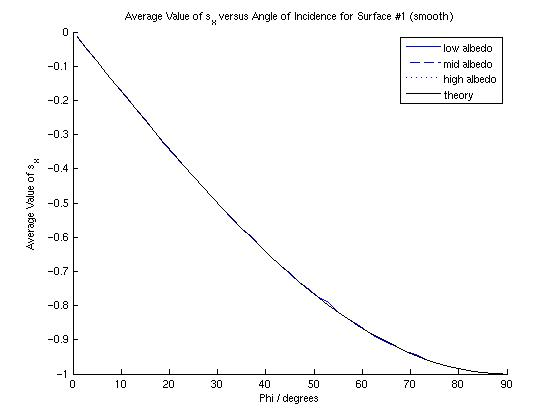
\includegraphics[width=95mm]{figs/sda/s_x_smooth.jpg}
        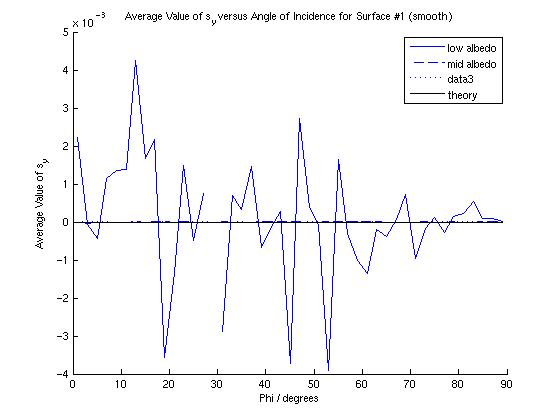
\includegraphics[width=95mm]{figs/sda/s_y_smooth.jpg}
        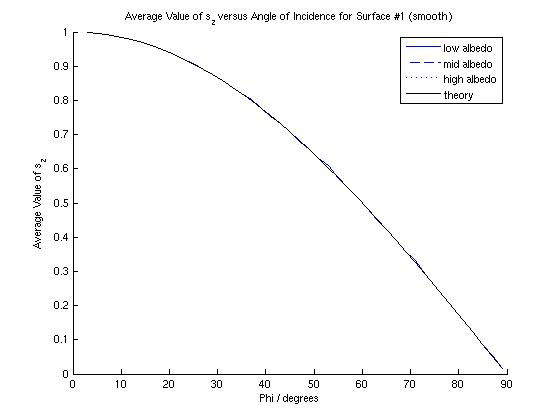
\includegraphics[width=95mm]{figs/sda/s_z_smooth.jpg}
        \caption{Analytical and numerical mean values for components of
                 the reflection vector from a smooth surface as a
                 function of incident angle}
        \label{fig:ivv_sda_s_vector}
      \end{figure}

      Figures~\ref{fig:ivv_sda_s_vector_diffs_x},
      ~\ref{fig:ivv_sda_s_vector_diffs_y},
      and~\ref{fig:ivv_sda_s_vector_diffs_z} show the differences
      along each axis for each of the four surfaces shown in
      Figure~\ref{fig:ivv_surface_profiles}.

      \begin{figure}[!ht]
        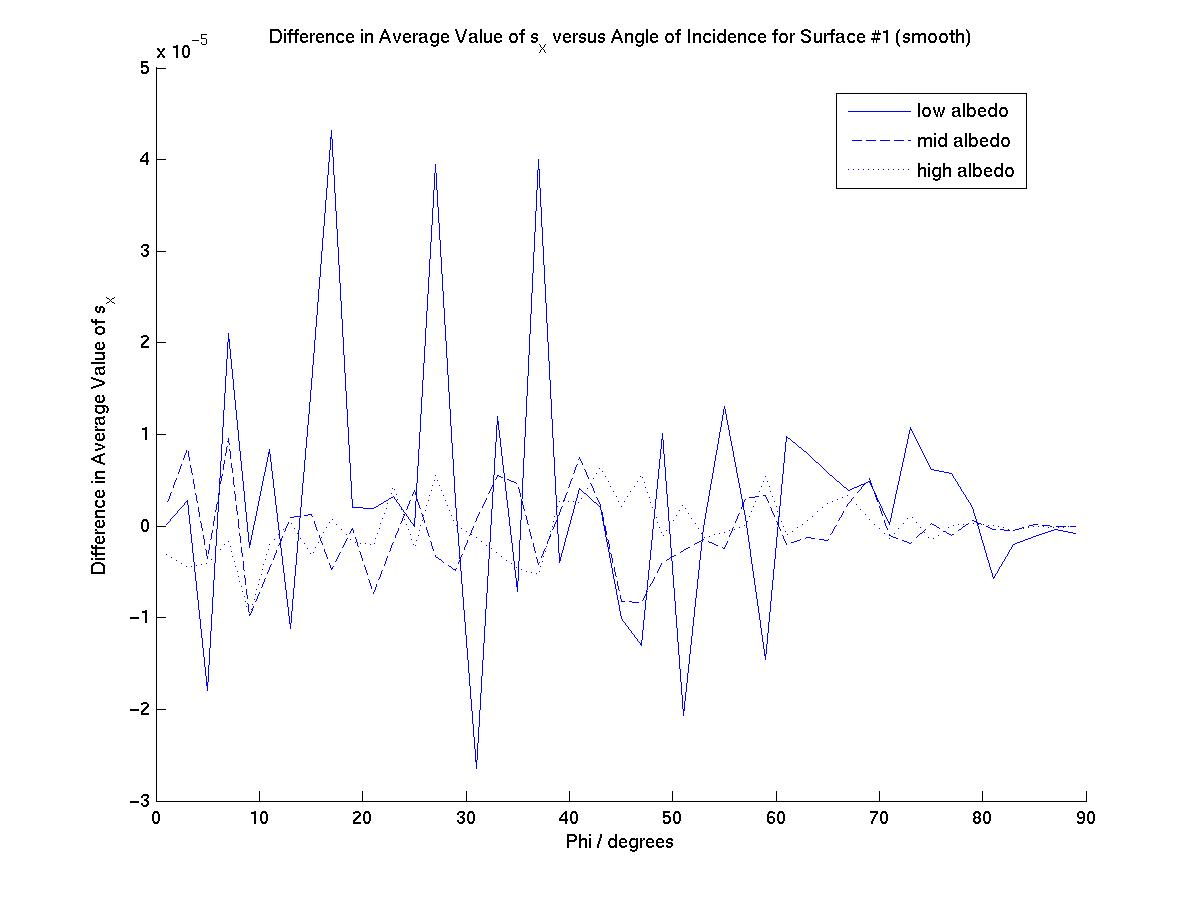
\includegraphics[width=95mm]{figs/sda/unit_vec_diff__x_smooth.jpg}
        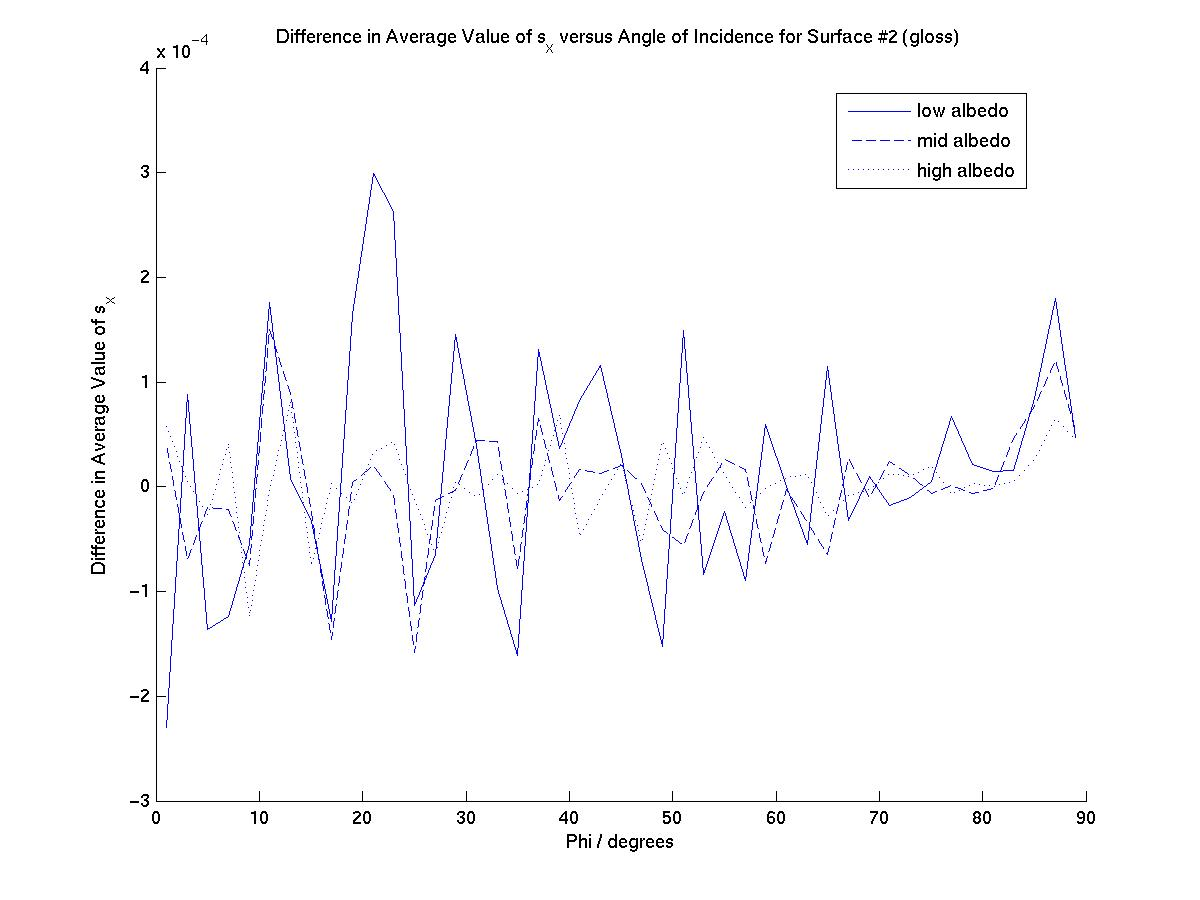
\includegraphics[width=95mm]{figs/sda/unit_vec_diff__x__gloss.jpg}
        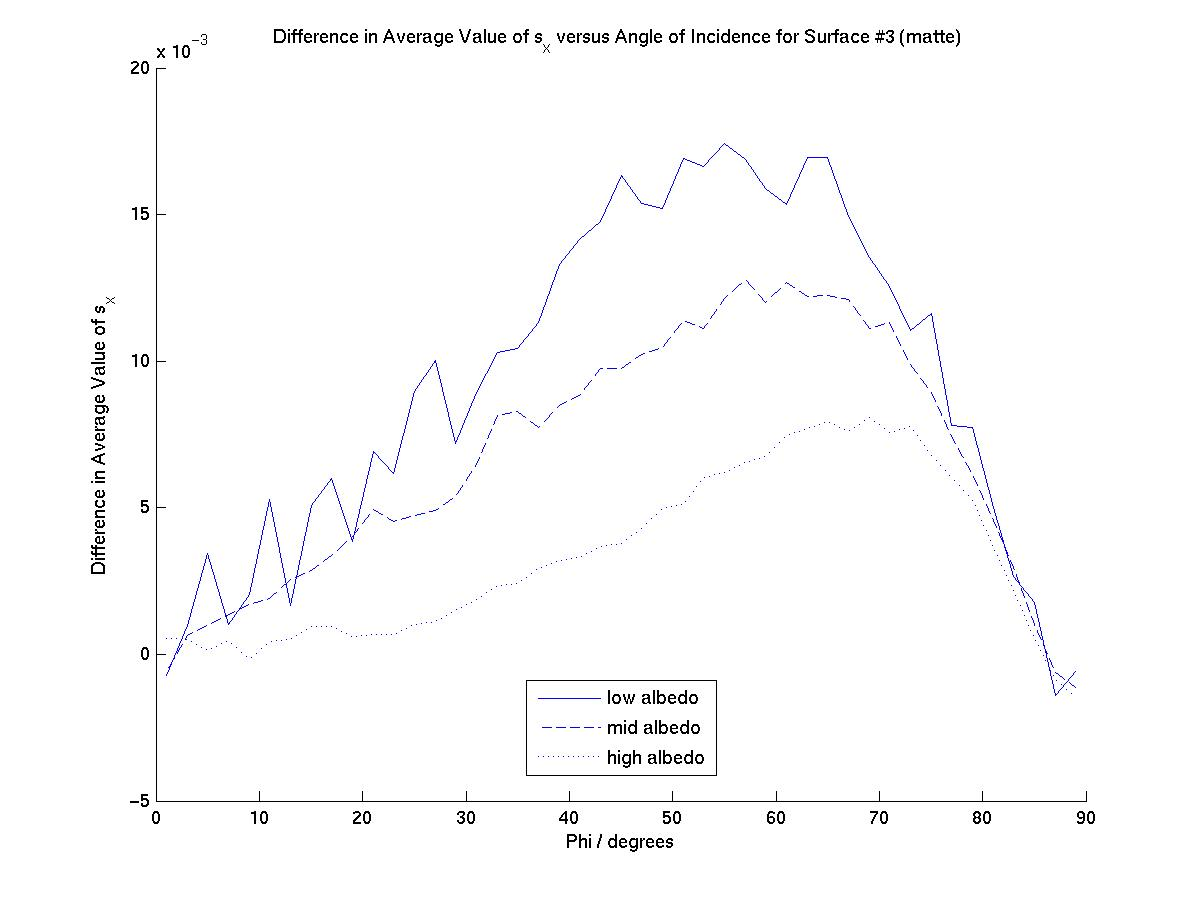
\includegraphics[width=95mm]{figs/sda/unit_vec_diff__x__matte.jpg}
        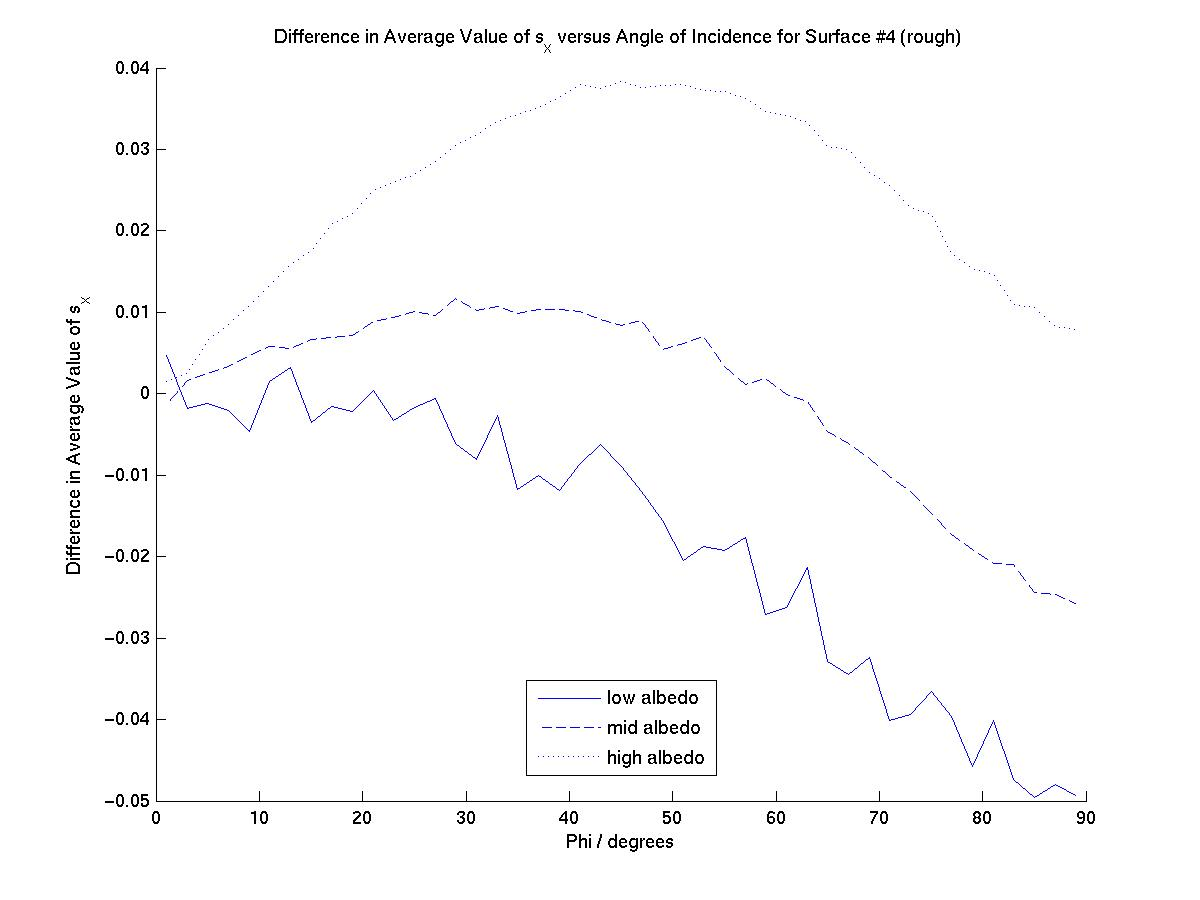
\includegraphics[width=95mm]{figs/sda/unit_vec_diff__x__rough.jpg}
        \caption{Differences between the analytic and numeric x-component of
                 $\langle \hat{s}\rangle$ for each of the 4
                 surface-profiles.}
        \label{fig:ivv_sda_s_vector_diffs_x}
      \end{figure}

      \begin{figure}[!ht]
        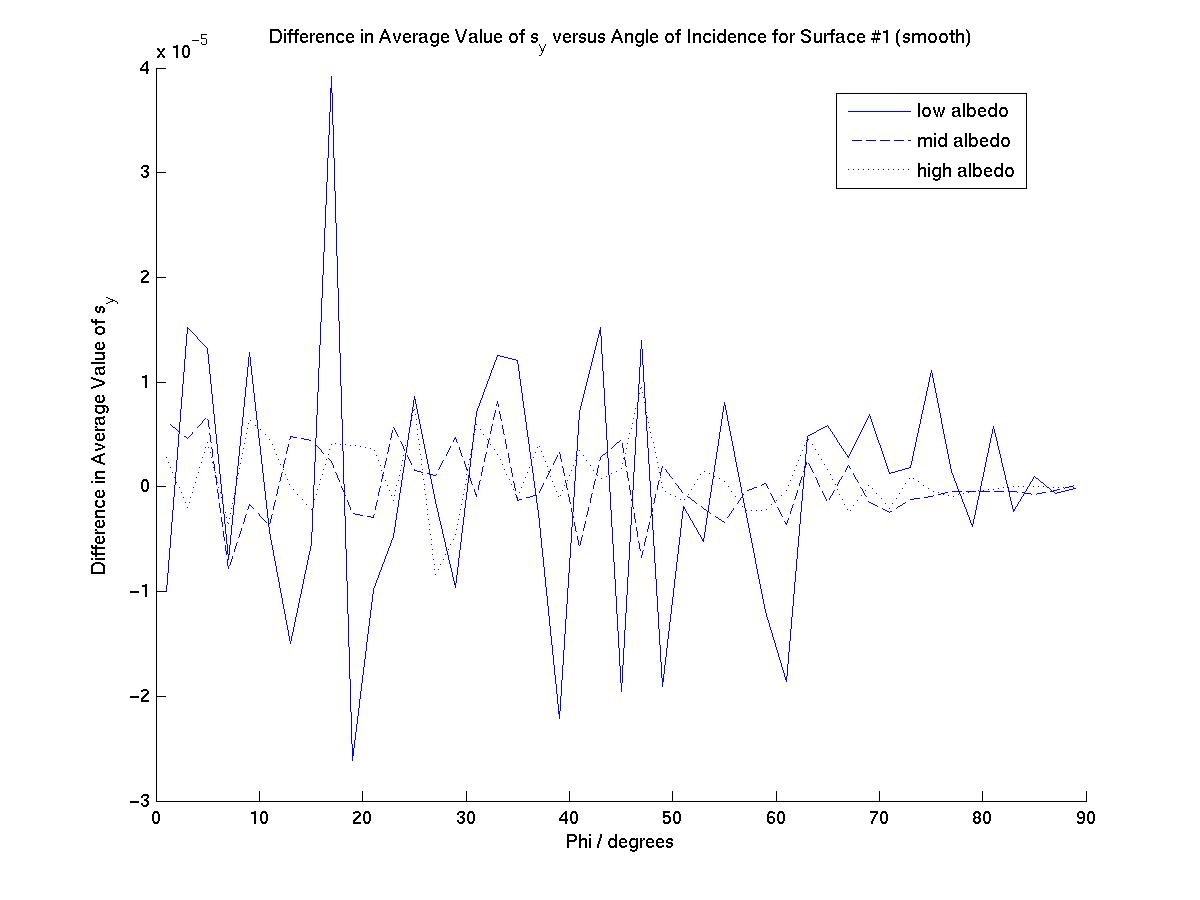
\includegraphics[width=95mm]{figs/sda/unit_vec_diff__y_smooth.jpg}
        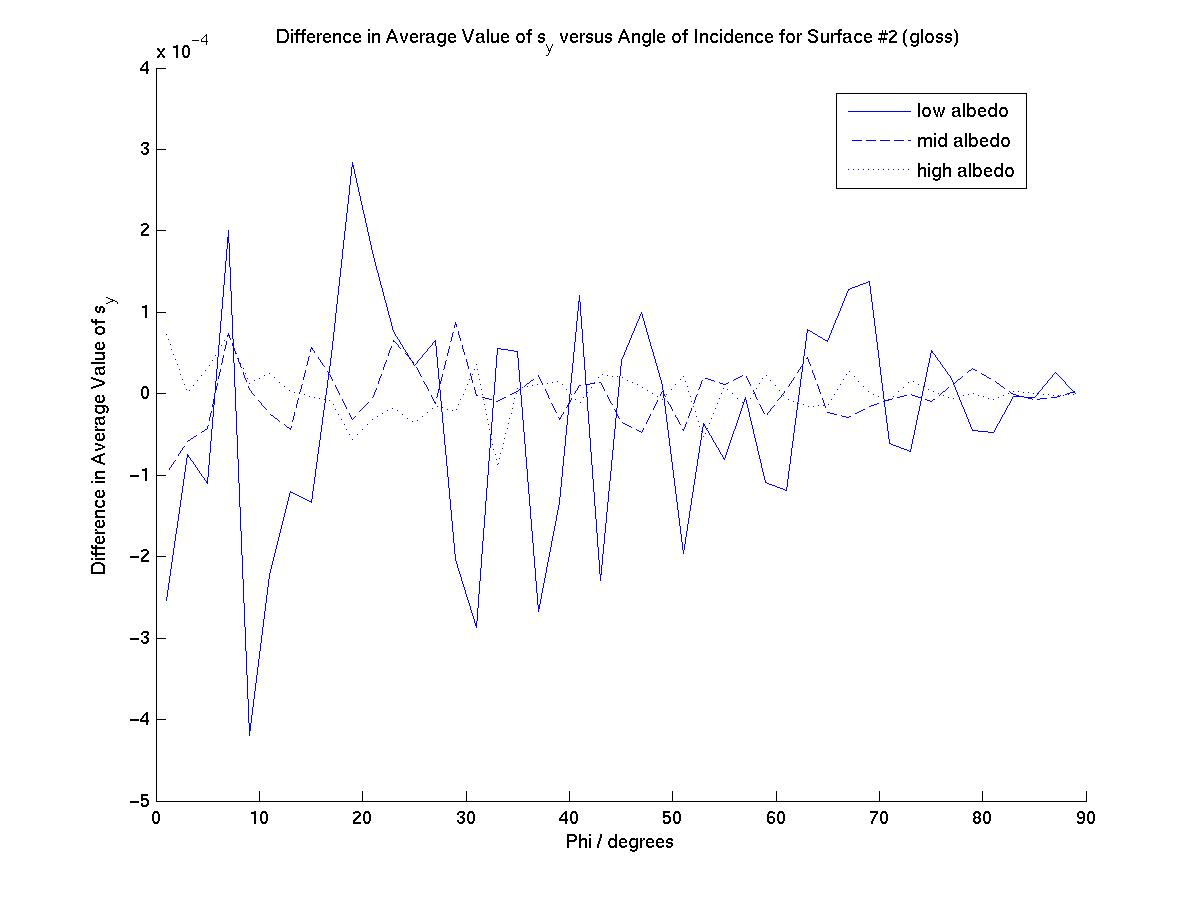
\includegraphics[width=95mm]{figs/sda/unit_vec_diff__y__gloss.jpg}
        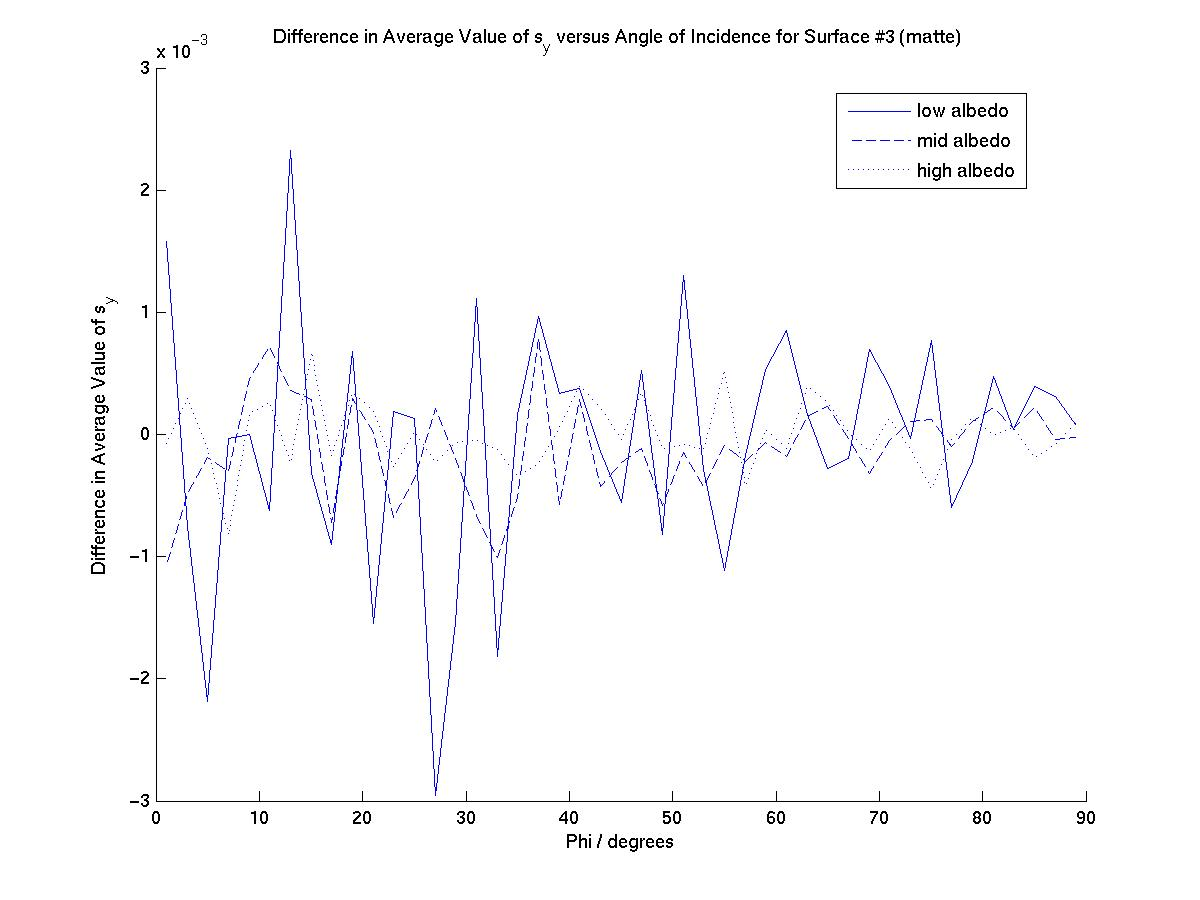
\includegraphics[width=95mm]{figs/sda/unit_vec_diff__y__matte.jpg}
        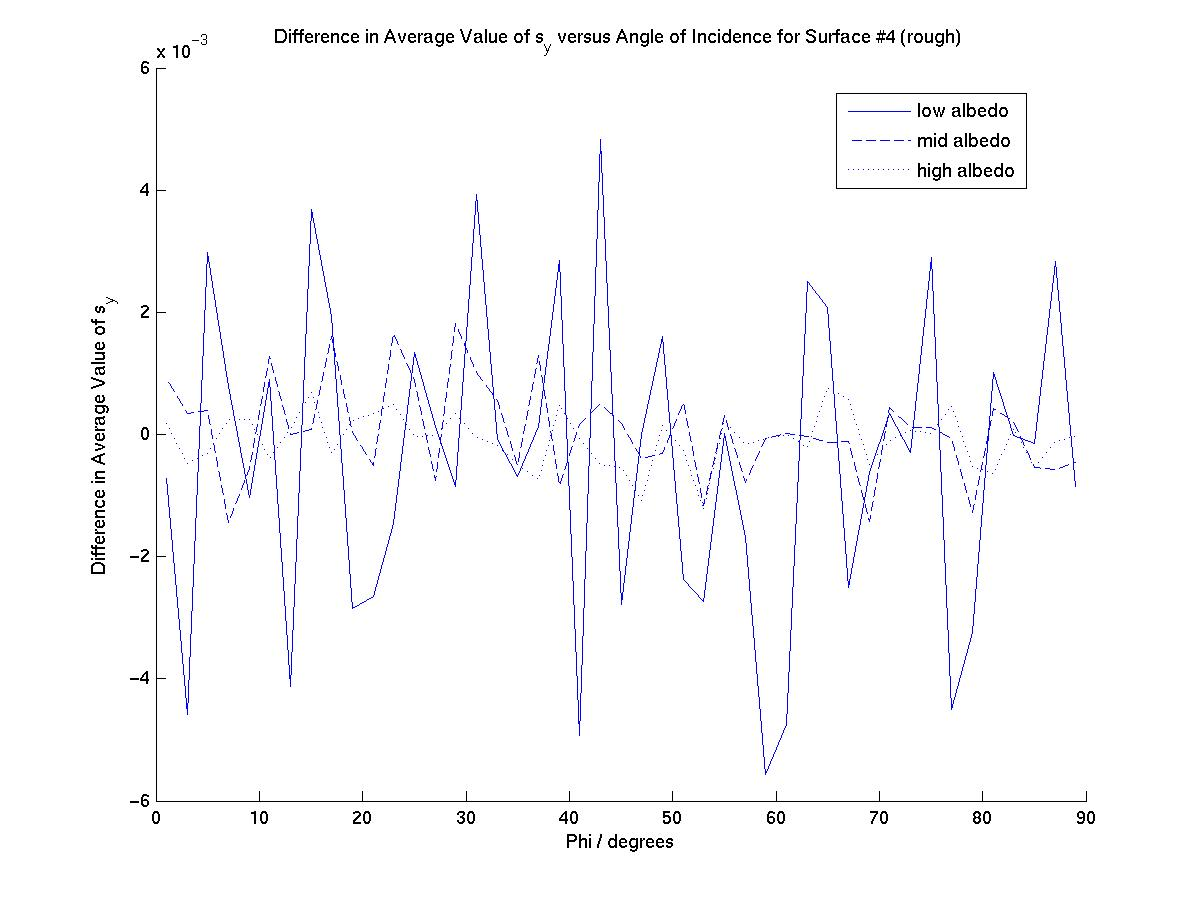
\includegraphics[width=95mm]{figs/sda/unit_vec_diff__y__rough.jpg}
        \caption{Differences between the analytic and numeric y-component of
                 $\langle \hat{s}\rangle$ for each of the 4
                 surface-profiles.}
        \label{fig:ivv_sda_s_vector_diffs_y}
      \end{figure}

      \begin{figure}[!ht]
        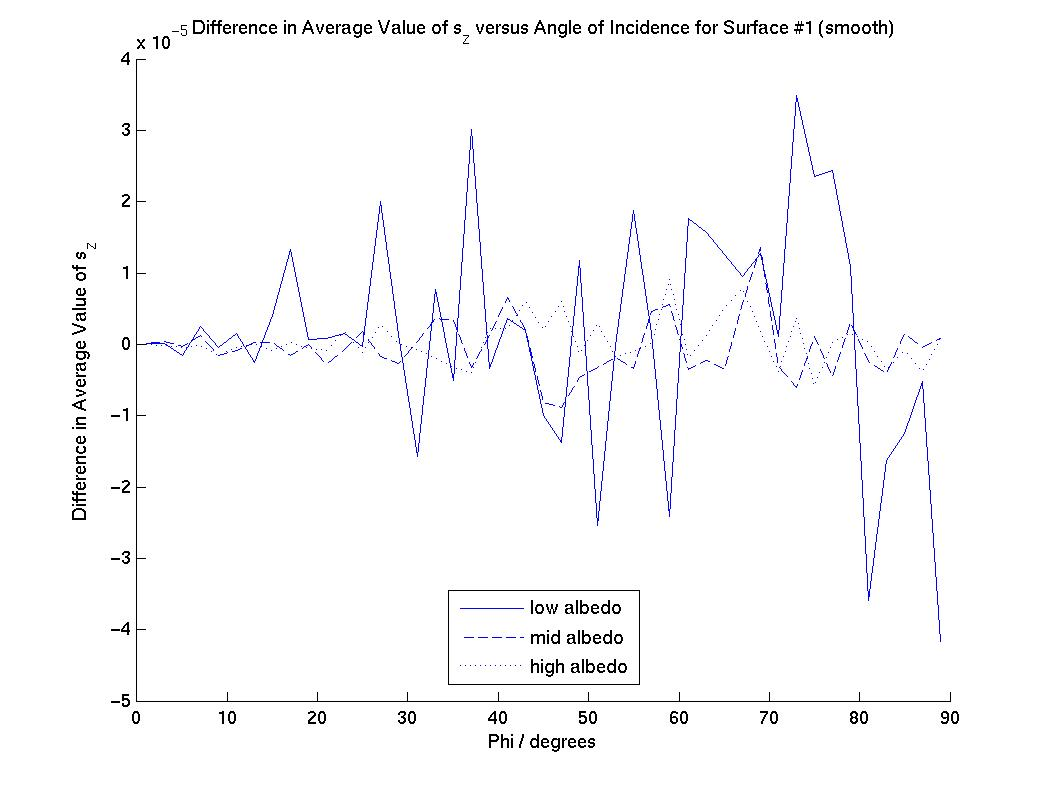
\includegraphics[width=95mm]{figs/sda/unit_vec_diff__z_smooth.jpg}
        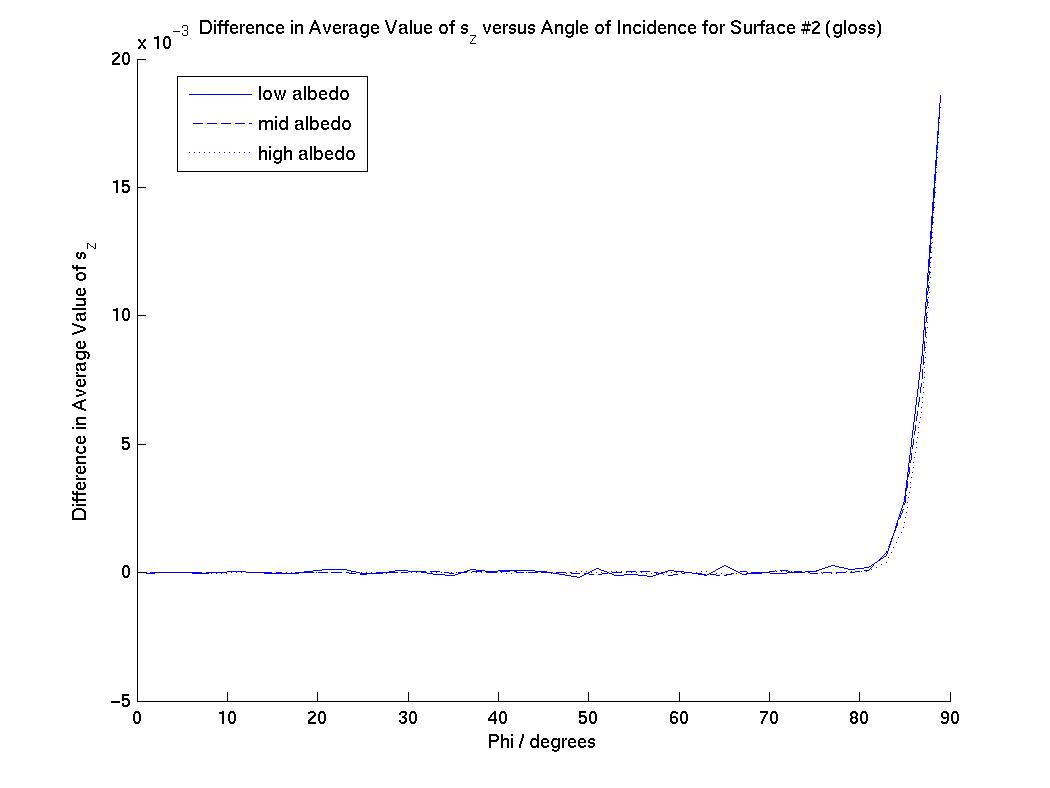
\includegraphics[width=95mm]{figs/sda/unit_vec_diff__z__gloss.jpg}
        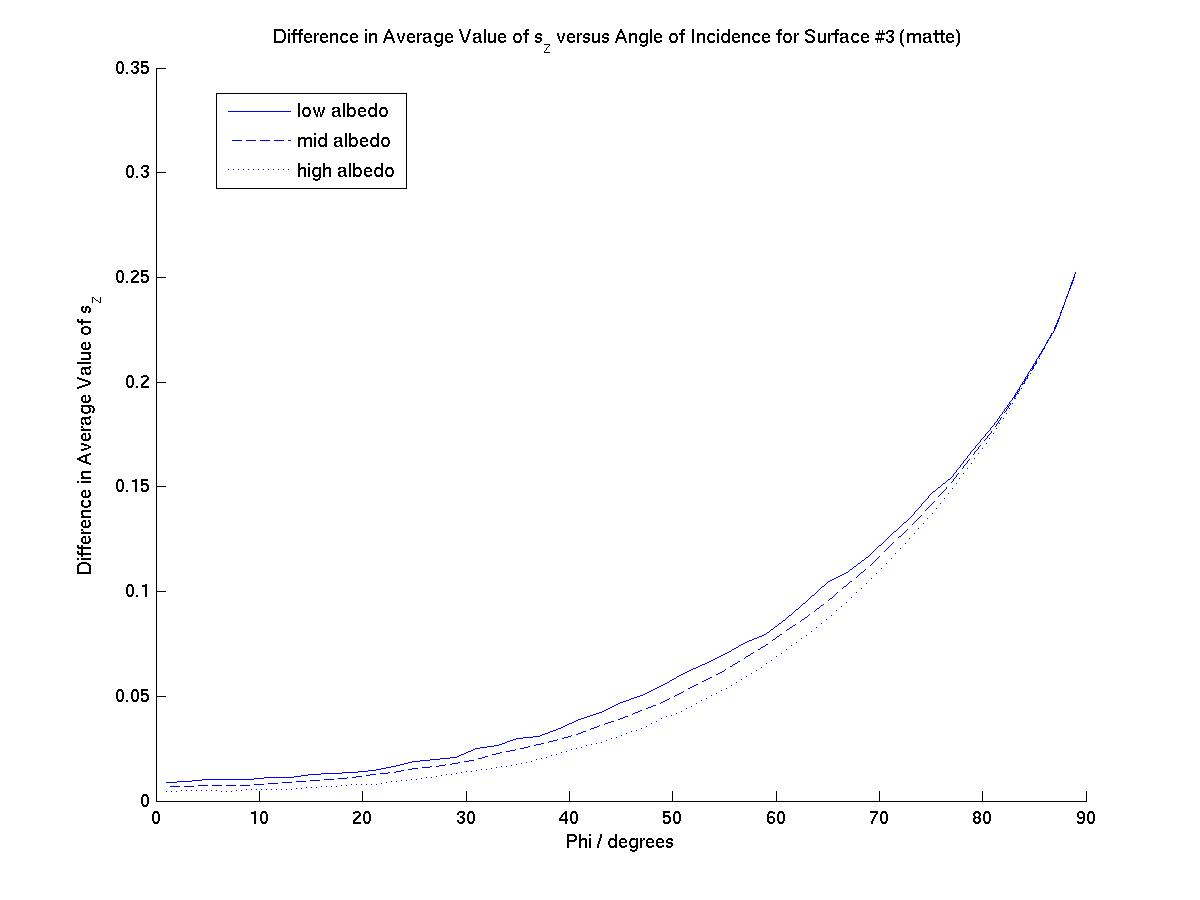
\includegraphics[width=95mm]{figs/sda/unit_vec_diff__z__matte.jpg}
        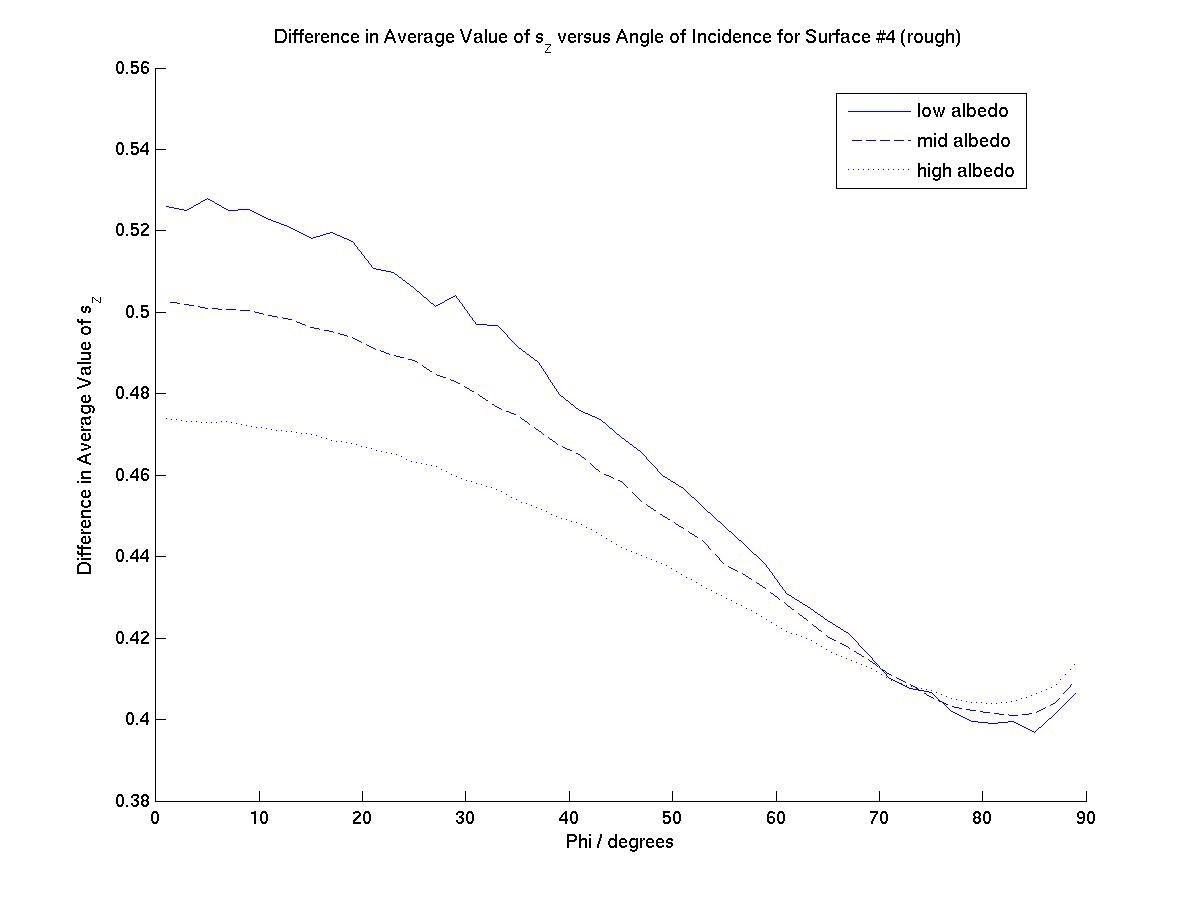
\includegraphics[width=95mm]{figs/sda/unit_vec_diff__z__rough.jpg}
        \caption{Differences between the analytic and numeric z-component of
                 $\langle \hat{s}\rangle$ for each of the 4
                 surface-profiles.}
        \label{fig:ivv_sda_s_vector_diffs_z}
      \end{figure}

      \clearpage

     \subsection{Force Comparisons}
      For each angle of incidence, the total force calculated by
      each of the two models can be expressed as:
      \begin{enumerate}
        \item{}Numerical Model
          \begin{equation}
            {\vec{F}}_{\mathit{num}}=\sum _{i=1}^{N}\vec{\mathit{dF}}_{i}
            \label{eqn:ivv_fvi_force_numerical}
          \end{equation}

          where \newline
          \begin{itemize}
            \item{}
              $\vec{\mathit{dF}}_{i}=
                \begin{cases}
                  f_{\gamma }\left(-\hat{p}-\hat{s}_{i}\right) &
                    \mathit{photon~ is~ reflected}\\
                  f_{\gamma }\left(-\hat{p}-\frac{2}{3}\hat{k}\right) &
                    \mathit{photon~ is~
                    absorbed~and~re-emitted,~or~reflected~diffusely}
                \end{cases}$
            \item{}
              $\hat{p}$,$\hat{s}$, and $\hat{k}$ are unit vectors for the
              incident radiation, specular reflection, and surface-normal
              vectors (Note:  $\hat{p}$ is directed \it against \rm the flux
              vector, away from the surface).
            \item{}
              $f_{\gamma }$ represents the ``force'' associated with the
              momentum of each incident photon per unit time.
            \item{}
              \textit{N} represents the number of ``photons'' being
              used.
          \end{itemize}

        \item{}Simplifying Model
          \begin{equation}
            {\vec{F}}_{\mathit{model}}=Nf_{\gamma }\left(-\hat{p}-\alpha
            (1-\delta)\hat{s}-\frac{2}{3}(1-\alpha (1-\delta ))\hat{k}\right)
            \label{eqn:ivv_fvi_force_simple}
          \end{equation}

          where  $\alpha $ and  $\delta $ represent the fraction of incident
          light that is reflected, and the fraction of the reflected
          light that is reflected diffusely.

      \end{enumerate}
      Equation~\ref{eqn:ivv_fvi_force_numerical} is evaluated
      for each angle of incidence, for each surface by calculating the force
      from each photon, and summing to provide the total force in
      each direction.

      For any given surface, the force is calculated for a number of incident
      angles, then the values  $\alpha $ and  $\delta $,  that provide the
      best fit ---  across all of those angles --- between
      equations ~\ref{eqn:ivv_fvi_force_numerical}
      and ~\ref{eqn:ivv_fvi_force_simple}, are
      determined.

      First the difference, \it per photon, \rm between
      equations~\ref{eqn:ivv_fvi_force_numerical}
      and~\ref{eqn:ivv_fvi_force_simple}
      is calculated for some angle of incidence ,  $\phi _{i} $ :

      \begin{equation}
        (\vec{{\Delta F}}_{\phi _{i} })=
        \frac{{\vec{F}}_{\mathit{num}}-{\vec{F}}_{\mathit{model}}}{N}
      \end{equation}

      The RMS value is used for determining ``best fit''.

      \begin{equation}
        \Delta F_{\mathit{RMS}}=\sqrt{\frac{1}{n}\sum _{i=1}^{n}|\vec{{\Delta
        F}}_{\phi _{i}}|^{2}}
      \end{equation}

      where \it n \rm represents the number of angles of incidence
      used in the numerical simulation.

      The contribution to this value from each axis are
      also calculated for analysis.

      \begin{equation}
        \Delta F_{x}=\sqrt{\frac{1}{n}\sum _{i=1}^{n}\left((\vec{{\Delta
        F}}_{\phi _{i}})\cdot \hat{i}\right)^{2}}
      \end{equation}

      \begin{equation}
        \Delta F_{y}=\sqrt{\frac{1}{n}\sum _{i=1}^{n}\left((\vec{{\Delta
        F}}_{\phi _{i}})\cdot \hat{j}\right)^{2}}
      \end{equation}

      \begin{equation}
        \Delta F_{z}=\sqrt{\frac{1}{n}\sum _{i=1}^{n}\left((\vec{{\Delta
        F}}_{\phi _{i}})\cdot \hat{k}\right)^{2}}
      \end{equation}


      Values of $\alpha $ and  $\delta $ which minimize  $\Delta
      F_{\mathit{RMS}}$ are now determined, and those values used in
      equation~\ref{eqn:ivv_fvi_force_simple} to obtain a ``best'' estimate of
      the variation with incident
      angle of the force. The comparison of the numerical simulation to the
      best fit is shown in figures~\ref{fig:ivv_sda_f_vector_diffs_x},
     ~\ref{fig:ivv_sda_f_vector_diffs_y}, and
     ~\ref{fig:ivv_sda_f_vector_diffs_z}.
      Note that in places, the best
      fit line is wholly above or below the data; this is because the data are
      showing 1 dimension at a time, whereas the best fit line is based on
      all dimensions together.

      \begin{figure}[!ht]
        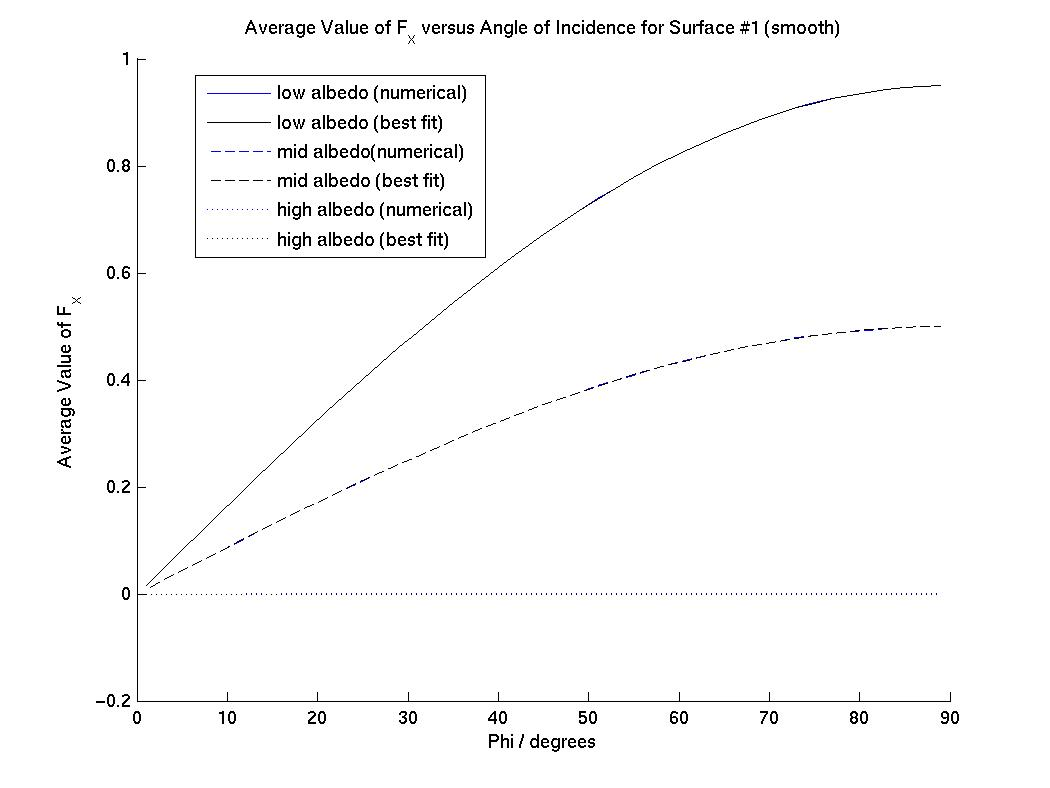
\includegraphics[width=95mm]{figs/sda/F__x_diff_smooth.jpg}
        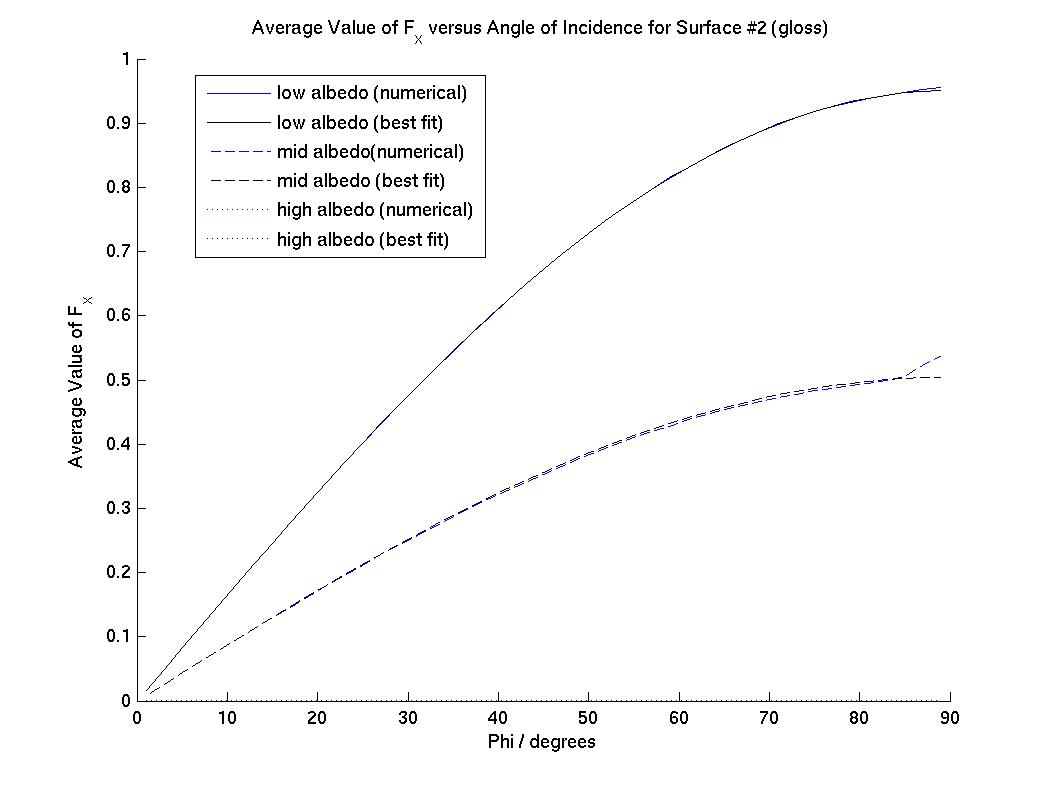
\includegraphics[width=95mm]{figs/sda/F__x_diff__gloss.jpg}
        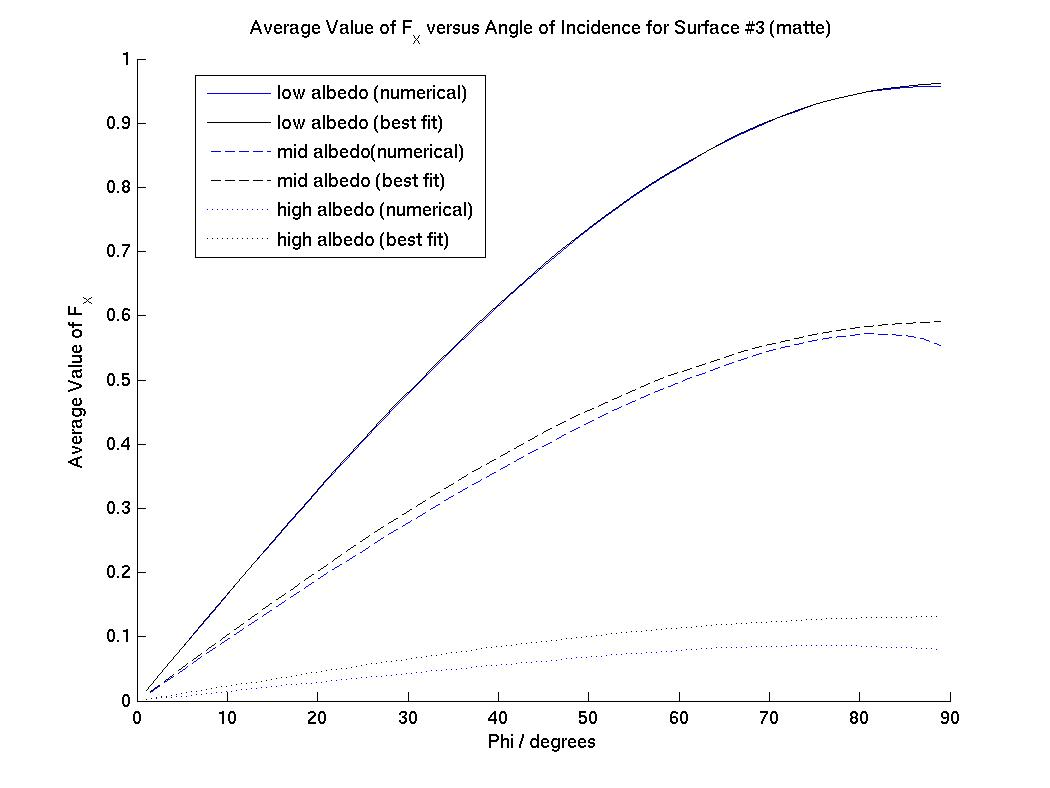
\includegraphics[width=95mm]{figs/sda/F__x_diff__matte.jpg}
        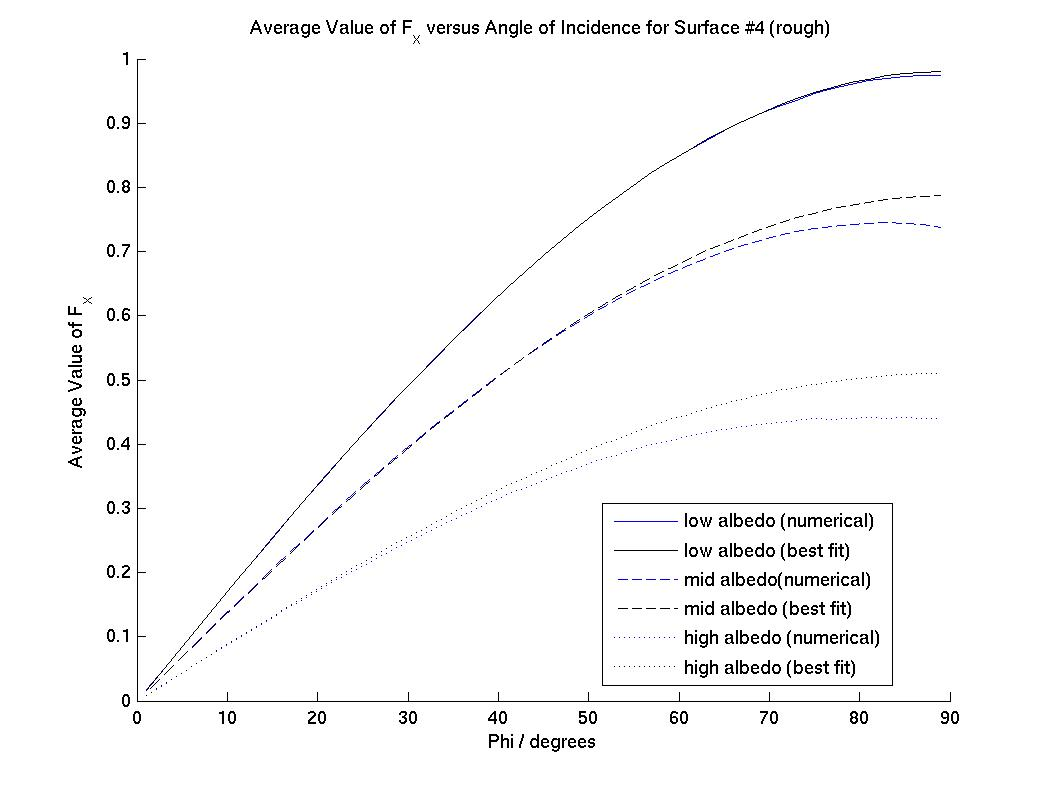
\includegraphics[width=95mm]{figs/sda/F__x_diff__rough.jpg}
        \caption{Mean values for the analytic and numeric x-component of
                the interaction force for each of the 4
                surface-profiles.}
        \label{fig:ivv_sda_f_vector_diffs_x}
      \end{figure}

      \begin{figure}[!ht]
        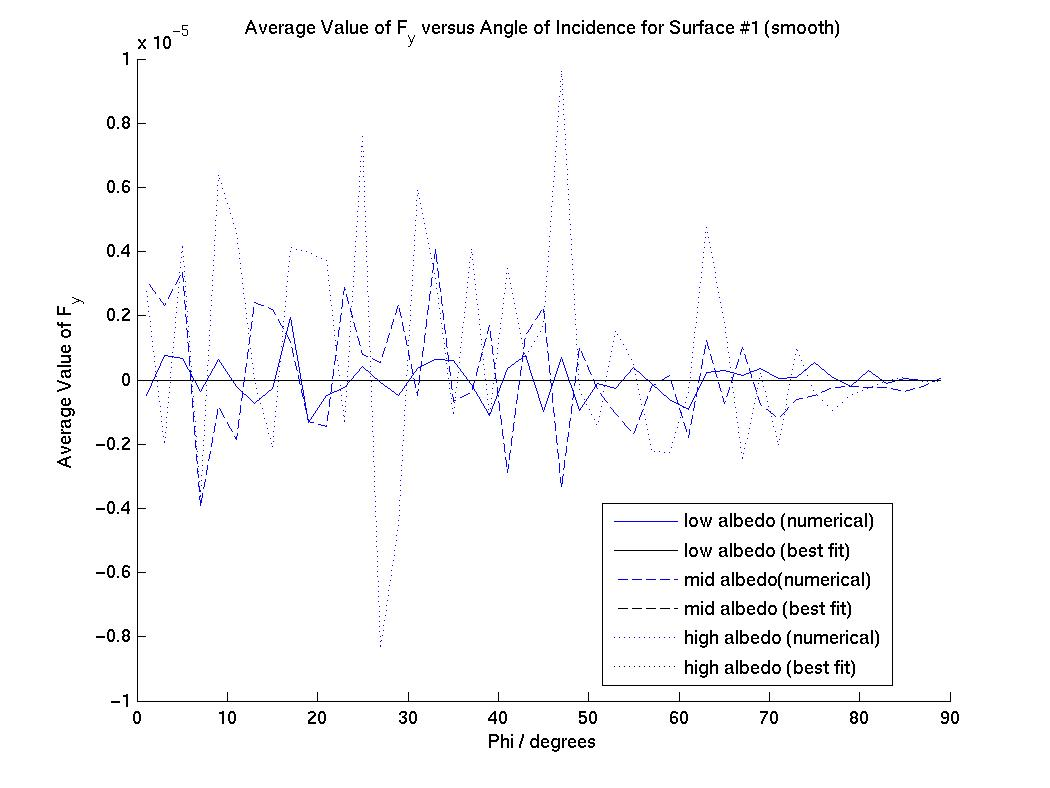
\includegraphics[width=95mm]{figs/sda/F__y_diff_smooth.jpg}
        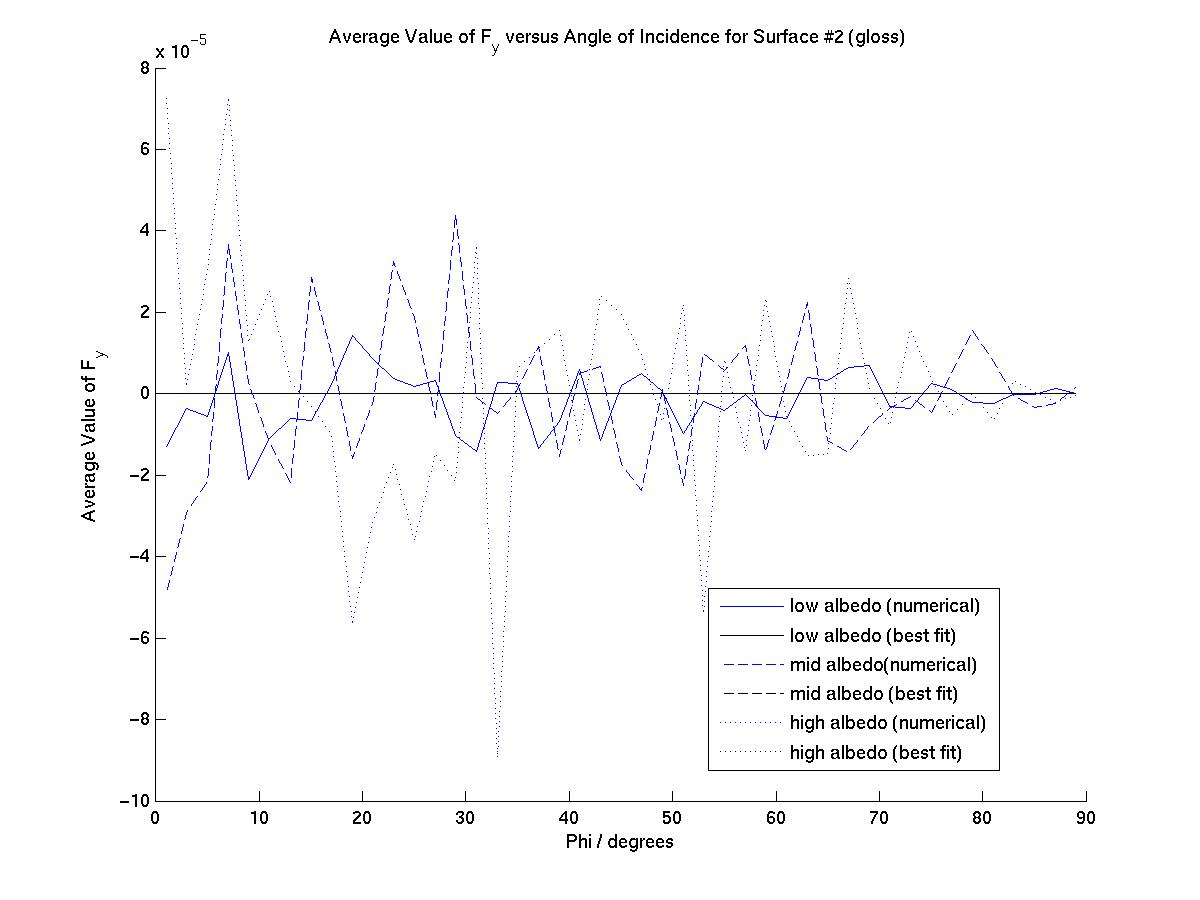
\includegraphics[width=95mm]{figs/sda/F__y_diff__gloss.jpg}
        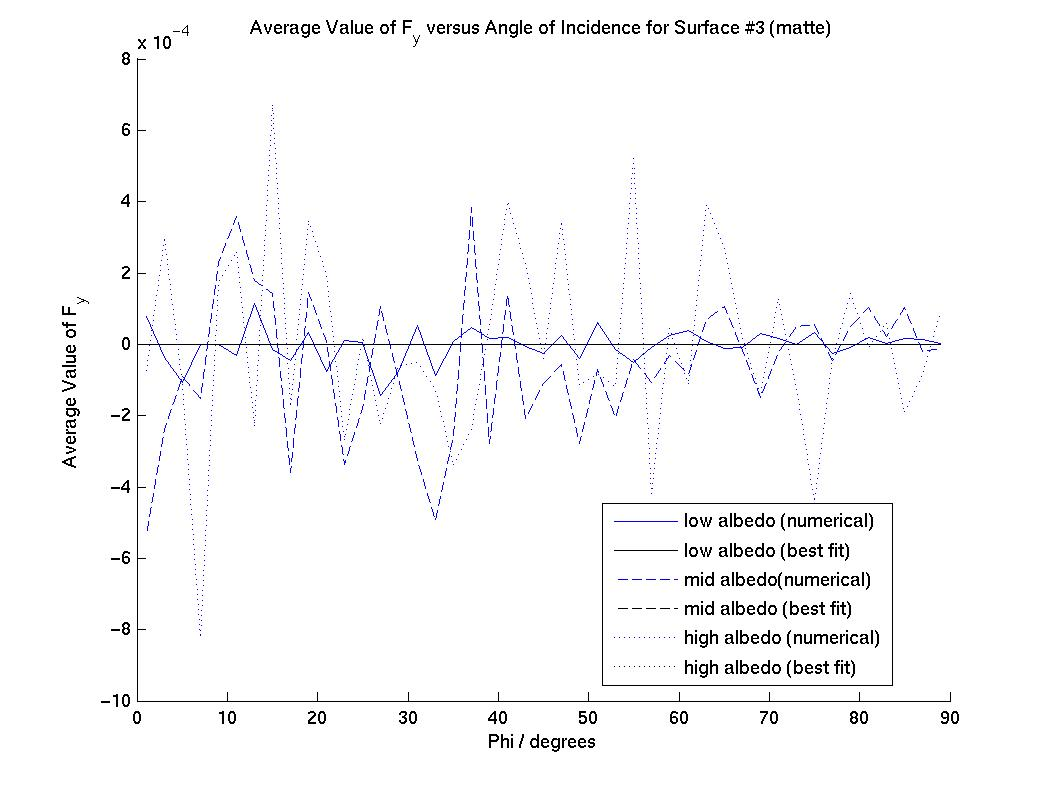
\includegraphics[width=95mm]{figs/sda/F__y_diff__matte.jpg}
        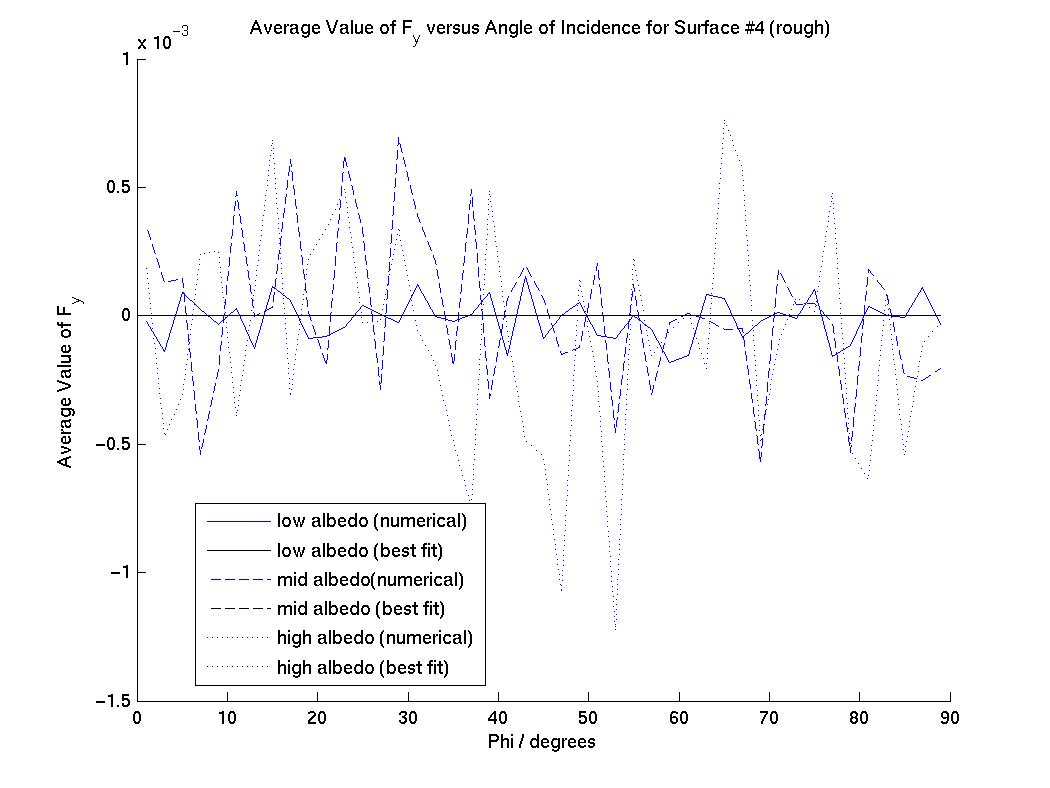
\includegraphics[width=95mm]{figs/sda/F__y_diff__rough.jpg}
        \caption{Mean values for the analytic and numeric y-component of
                the interaction force for each of the 4
                surface-profiles.}
        \label{fig:ivv_sda_f_vector_diffs_y}
      \end{figure}

      \begin{figure}[!ht]
        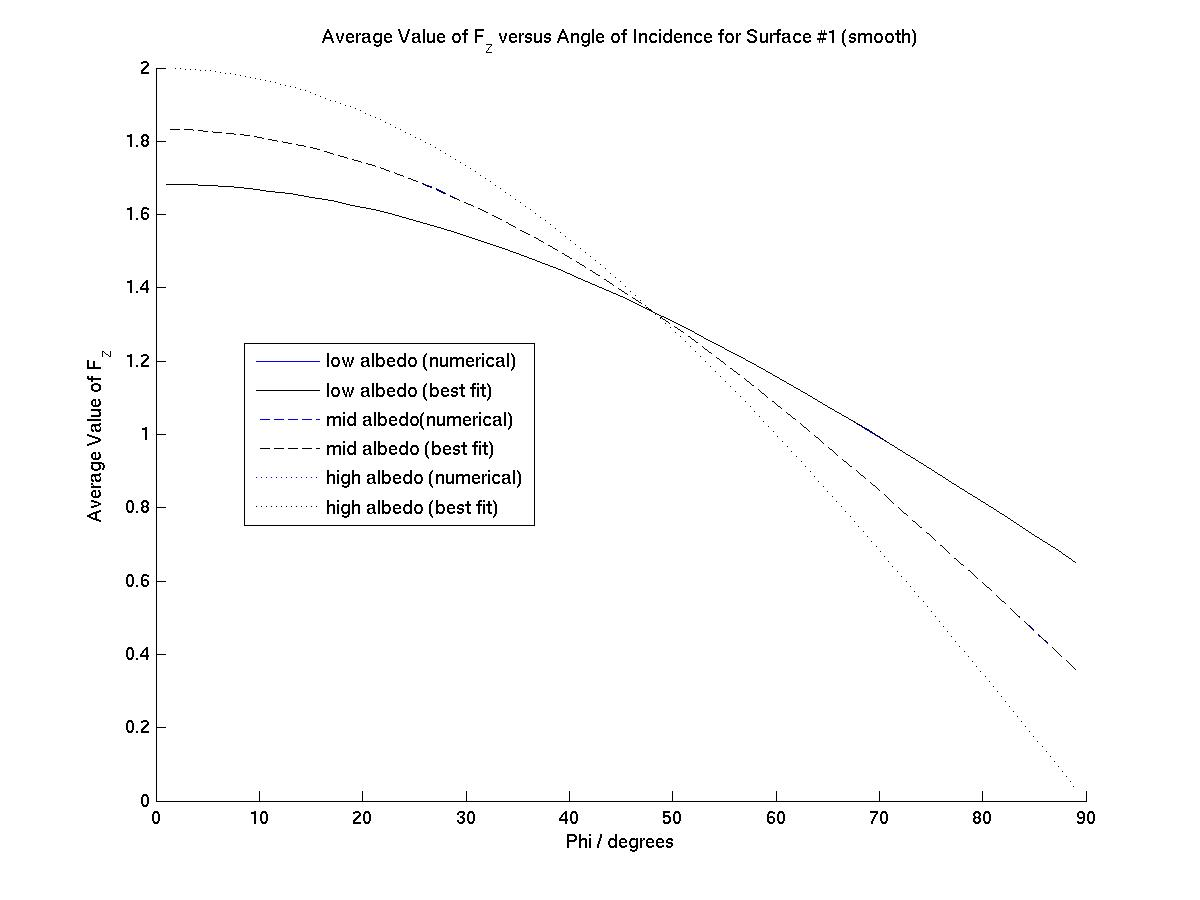
\includegraphics[width=95mm]{figs/sda/F__z_diff_smooth.jpg}
        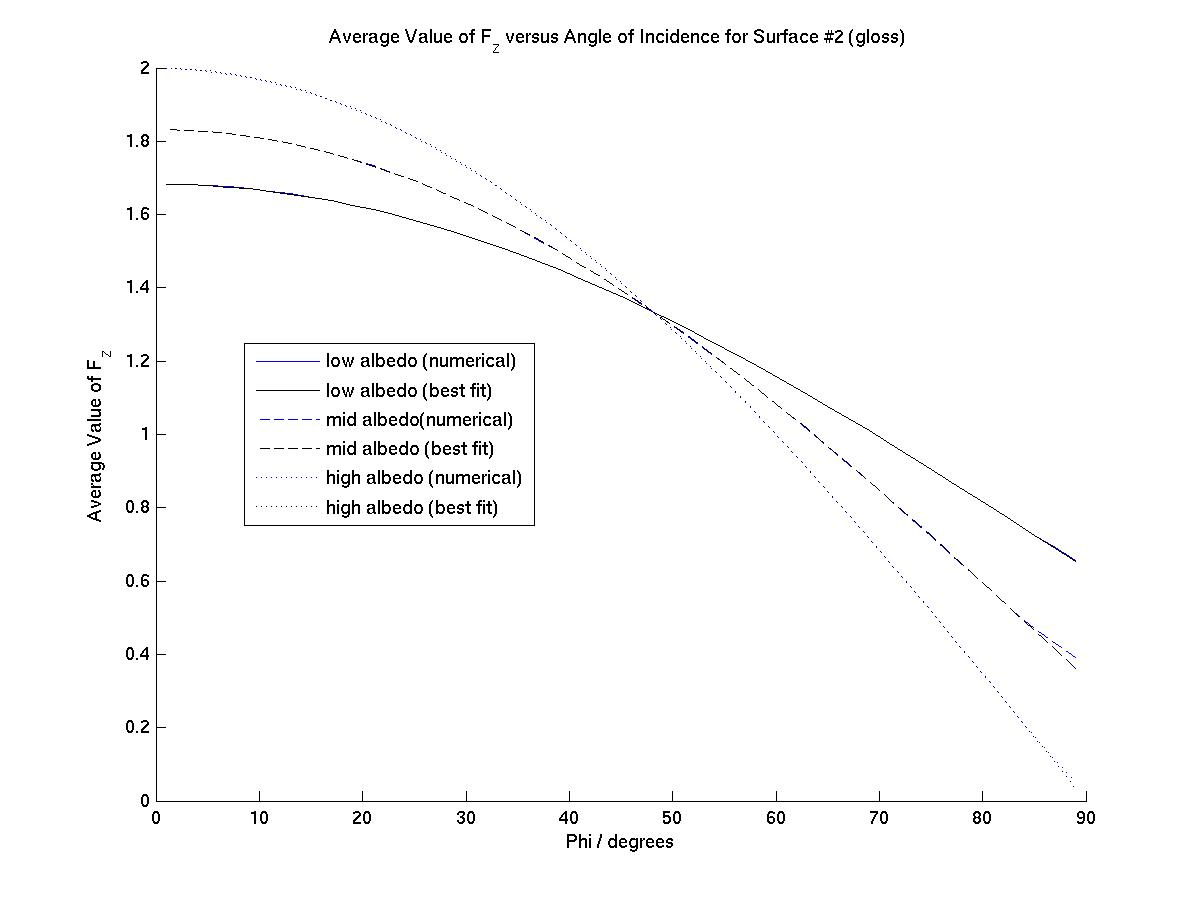
\includegraphics[width=95mm]{figs/sda/F__z_diff__gloss.jpg}
        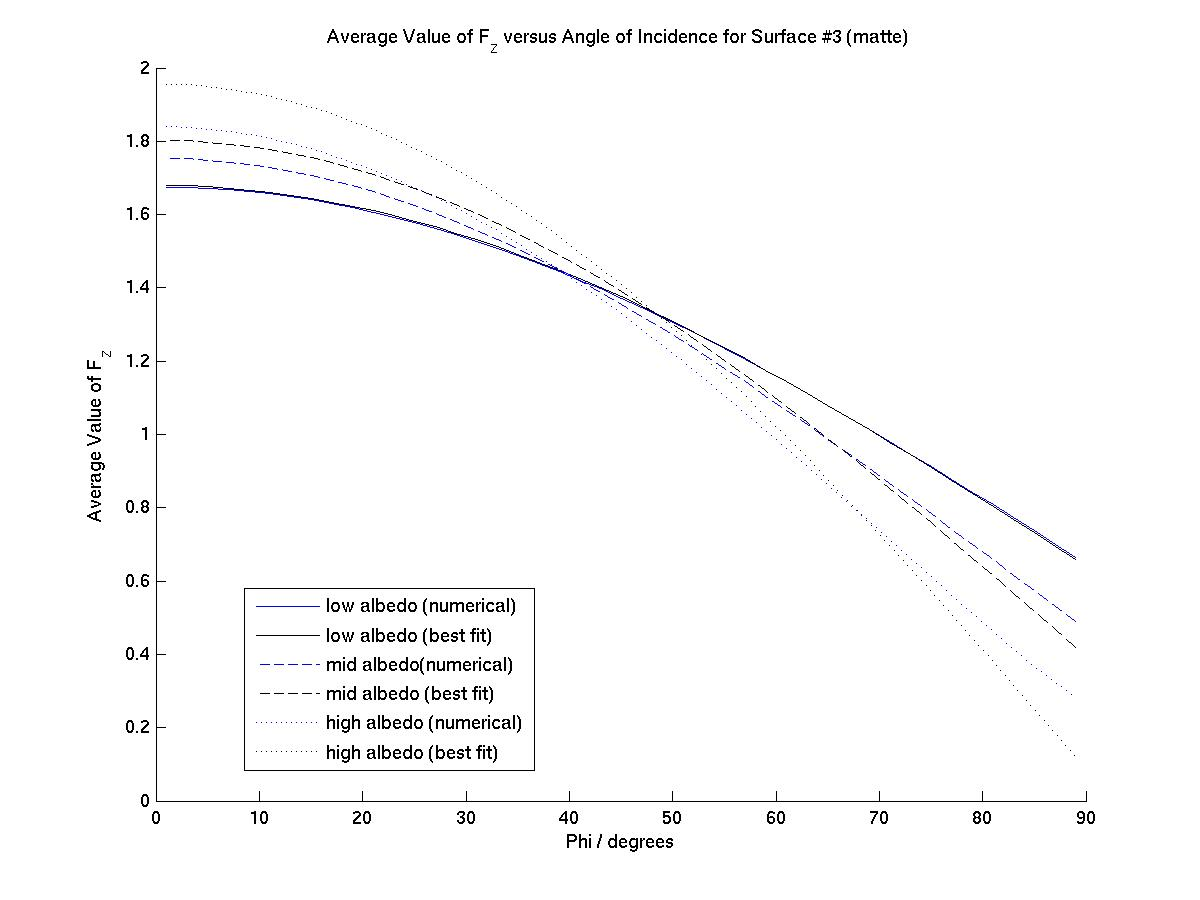
\includegraphics[width=95mm]{figs/sda/F__z_diff__matte.jpg}
        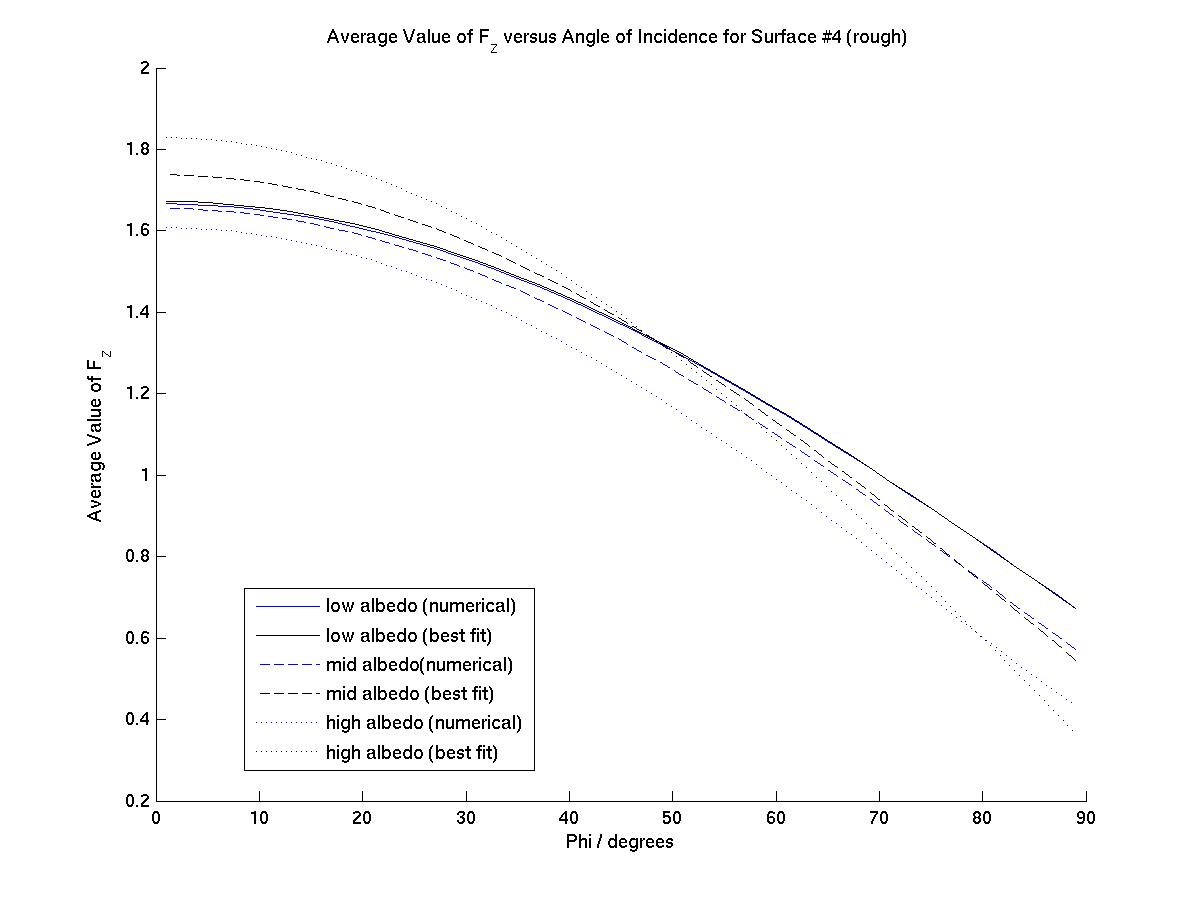
\includegraphics[width=95mm]{figs/sda/F__z_diff__rough.jpg}
        \caption{Mean values for the analytic and numeric z-component of
                the interaction force for each of the 4
                surface-profiles.}
        \label{fig:ivv_sda_f_vector_diffs_z}
      \end{figure}

      Notice that for all surfaces the behavior in the y-direction
      is small and unpredictable.
      For the smooth surface (surface \#1),
      the x{}- and z{}- components of the force behave
      as expected. In the x{}-direction, a highly reflective surface should
      produce no force, while a highly absorbent surface should absorb all of
      the momentum from the incident radiation, which varies as $\sin \phi$.
      In the z{}-direction, the highly reflective surface should
      experience a force of magnitude  $\cos \phi $ from each of incident and
      reflected radiation components, resulting in a curve that decreases from
      2 at
      $\phi =0$ to 0 at  $\phi =90$ degrees; the highly absorbent surface will
      experience the  $\cos \phi $ force from the incident radiation, and a
      force with magnitude 2/3 from the re{}-emitted radiation, causing the
      curve to fall from 1.67 to 0.67. The forces in the y{}-direction
      should be generally small compared with those in the x{}- and
      z{}-direction. These features are all observed. In all cases,
      values of $\alpha $ and  $\delta $ were found that provided a close fit
      between the numerical data and the simplified expression given in
      equation~\ref{eqn:ivv_fvi_force_simple}.

      \clearpage

      On closer inspection, under certain circumstances, the best fit of
      $\alpha $ and  $\delta $ to the data did not seem sensible. To
      investigate the degree to which the determination of the albedo and
      diffuse parameters are critical, plots have been generated showing the
      deviations  $\Delta F_{\mathit{RMS}}$ , $\Delta F_{x}$ and $\Delta
      F_{z}$ as functions of  $\alpha $ and  $\delta $ . An example of this
      may be seen on the error associated with a matte surface at medium
      albedo, which should have mid{}-range values for both  $\alpha $ and
      $\delta $ . From Figure~\ref{fig:ivv_sda_alpha_delta_F}, it is clear that
      appropriate values of
      0.6 and 0.4 respectively find the region of minimum error. However,
      the algorithmic search would not be able to distinguish between this,
      and values of 1.0 and 0.6 for  $\alpha $ and  $\delta $, which would
      be characteristic of a highly unusual surface that is both highly
      reflective and very rough.

      These data, presented in Figures~\ref{fig:ivv_sda_alpha_delta_F},
     ~\ref{fig:ivv_sda_alpha_delta_Fx}, and~\ref{fig:ivv_sda_alpha_delta_Fz},
      confirmed that ``sensible''
      values existed with very similar error even in those cases where the
      algorithmic search for lowest error produced unusual results. It is
      also apparent that there are a number of solutions of approximately
      equivalent merit, and that the determination of  $\alpha $ and  $\delta
      $ is probably not critical to better than 1 part in 10, and certainly
      not beyond 1 part in 100. At low albedo particularly, there is very little
      difference between the four surfaces, and making significant investment in a
      precise determination of $\alpha $ and  $\delta $ is futile.

      For
      reference on these figures, recall that the force{}-error is expressed
      \textit{per photon}, and that an error of value 1 is
      equivalent to the effect of the total incident radiation if it were all
      absorbed.
      The largest possible force-value on this scale is 2, which
      occurs in the vertical direction when $\phi =0$,
      and $\alpha =1$ on a perfectly smooth surface.

      This observation is further supported by data presented in
      section~\ref{test:plate_model},
      Figures~\ref{fig:ivv_platemod_fig1} to~\ref{fig:ivv_platemod_specdiff}.
      While the two
      types of reflection produce Force-time graphs with very different
      patterns, the integration of those graphs yields impulses that are quite
      similar.

  \begin{figure}[!ht]
  \leftskip=-20mm
  \begin{minipage}[t]{200mm}\centering
    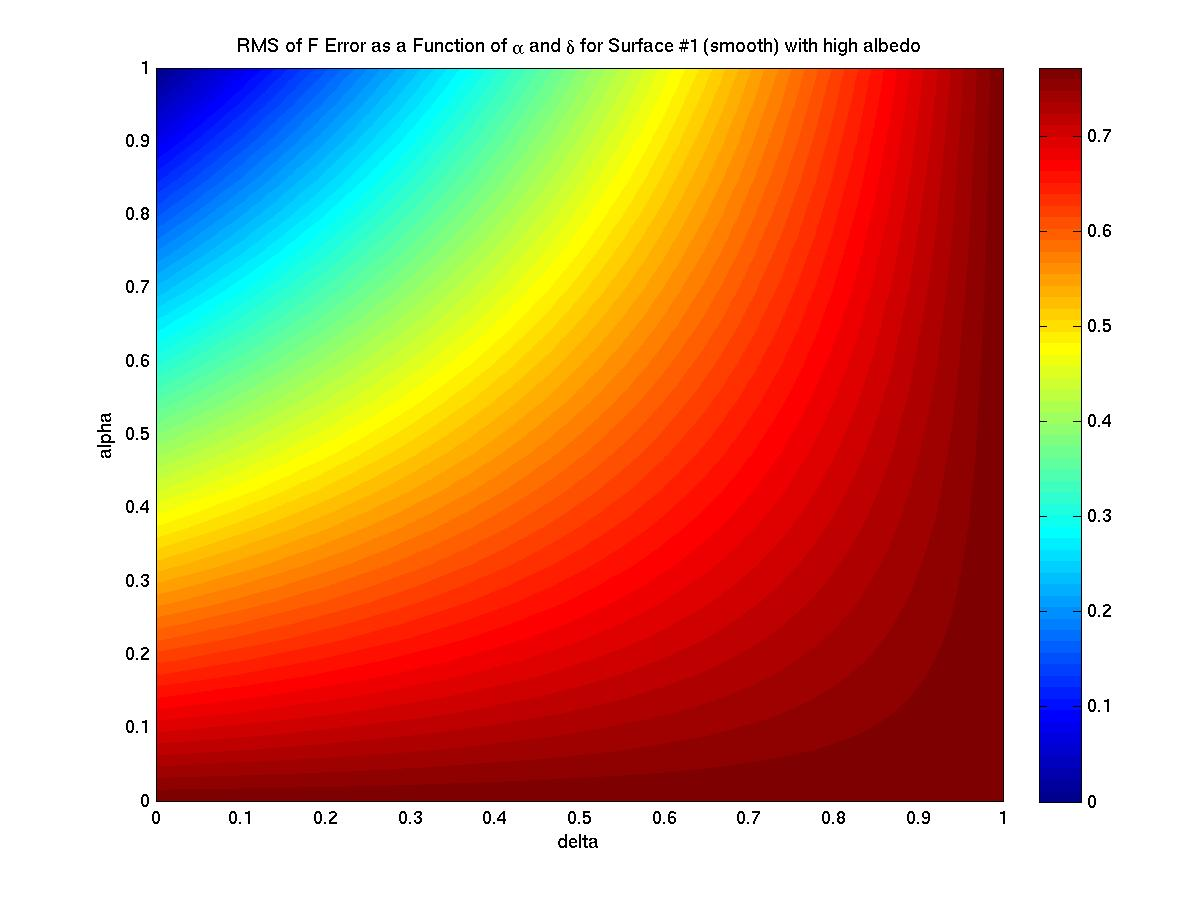
\includegraphics[width=65mm]{figs/sda/F_error_albedo_high_surf_smooth.jpg}
    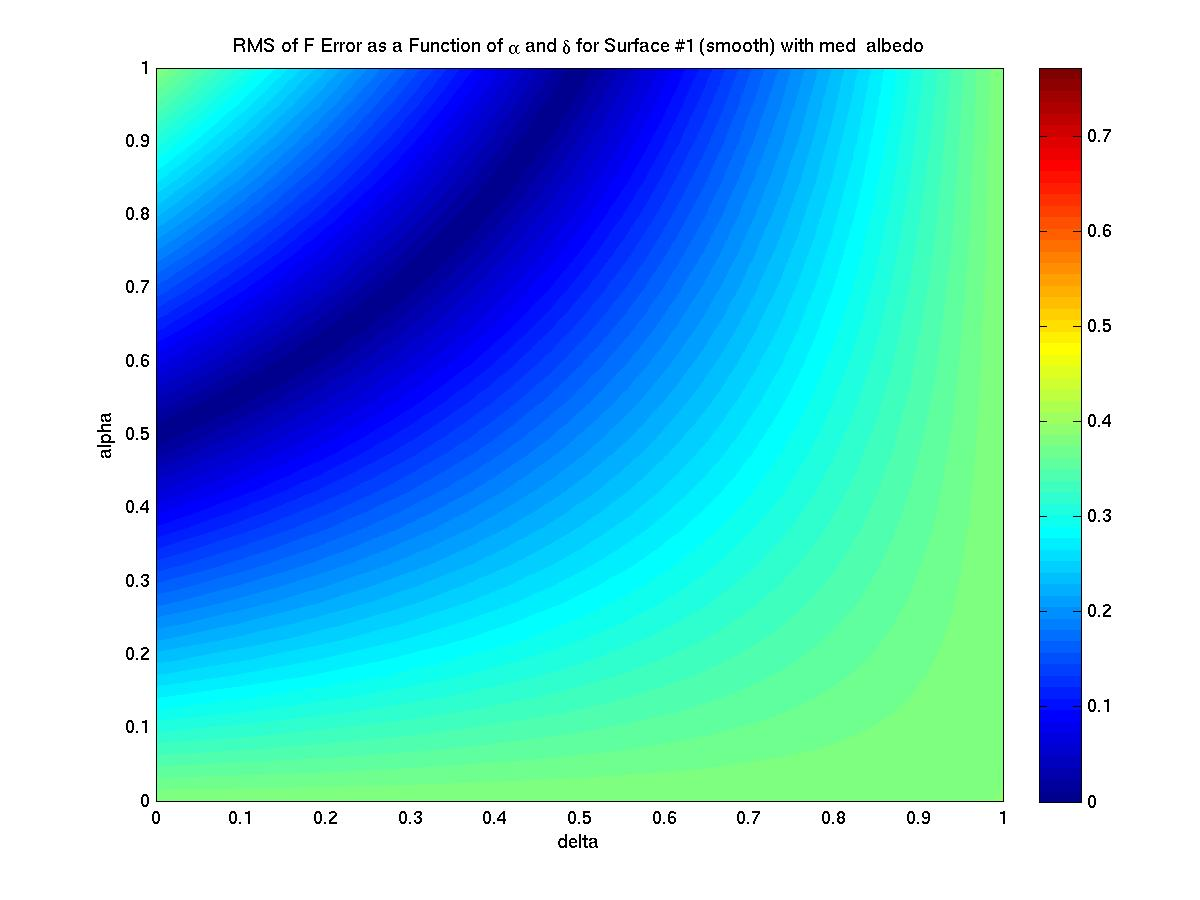
\includegraphics[width=65mm]{figs/sda/F_error_albedo__med_surf_smooth.jpg}
    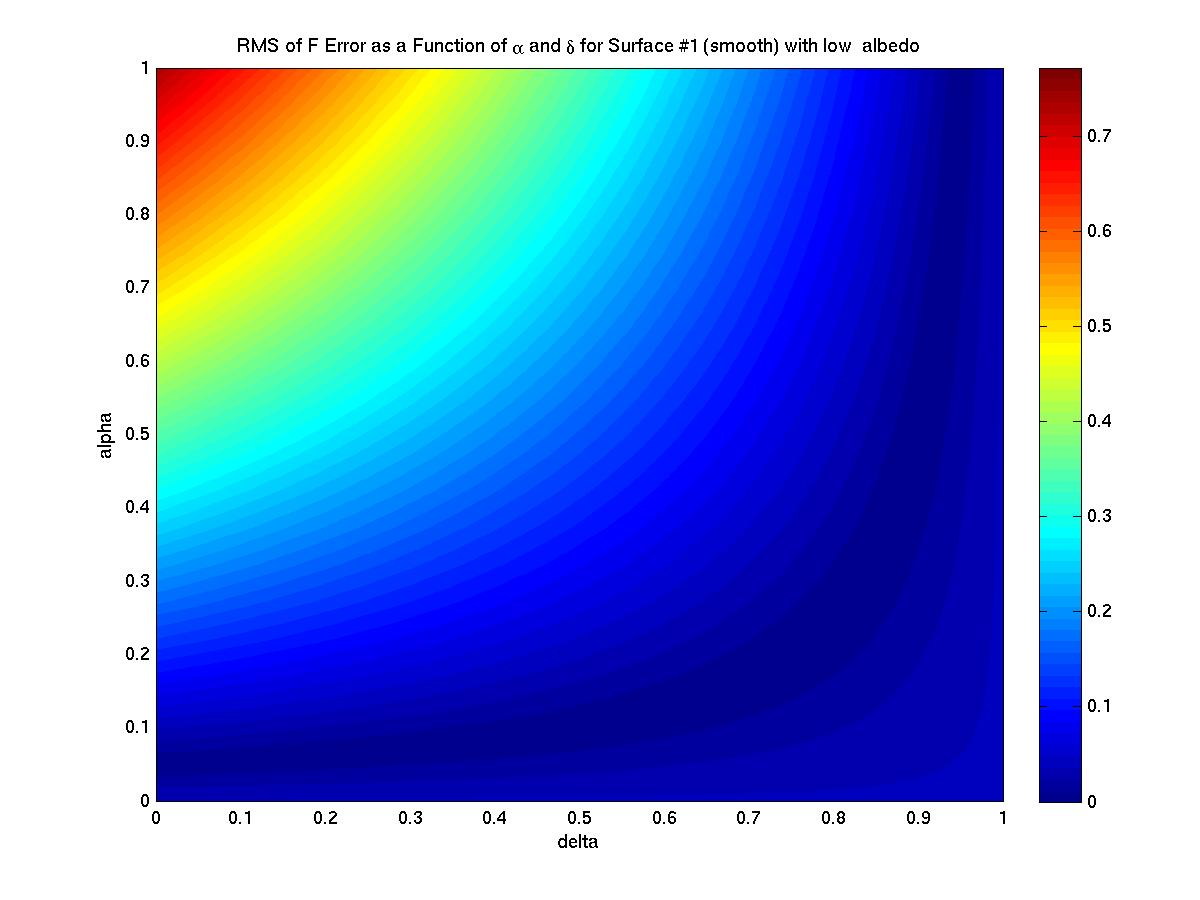
\includegraphics[width=65mm]{figs/sda/F_error_albedo__low_surf_smooth.jpg}
    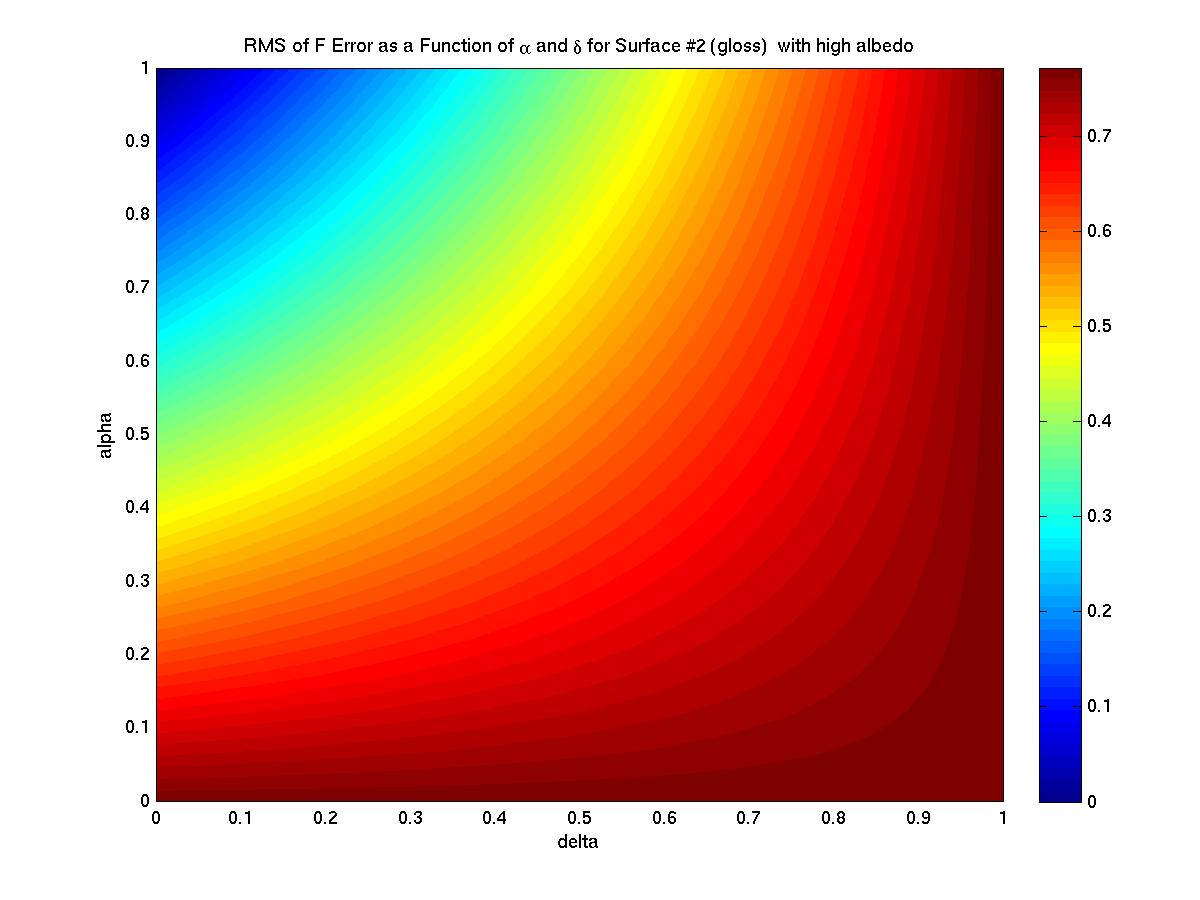
\includegraphics[width=65mm]{figs/sda/F_error_albedo_high_surf__gloss.jpg}
    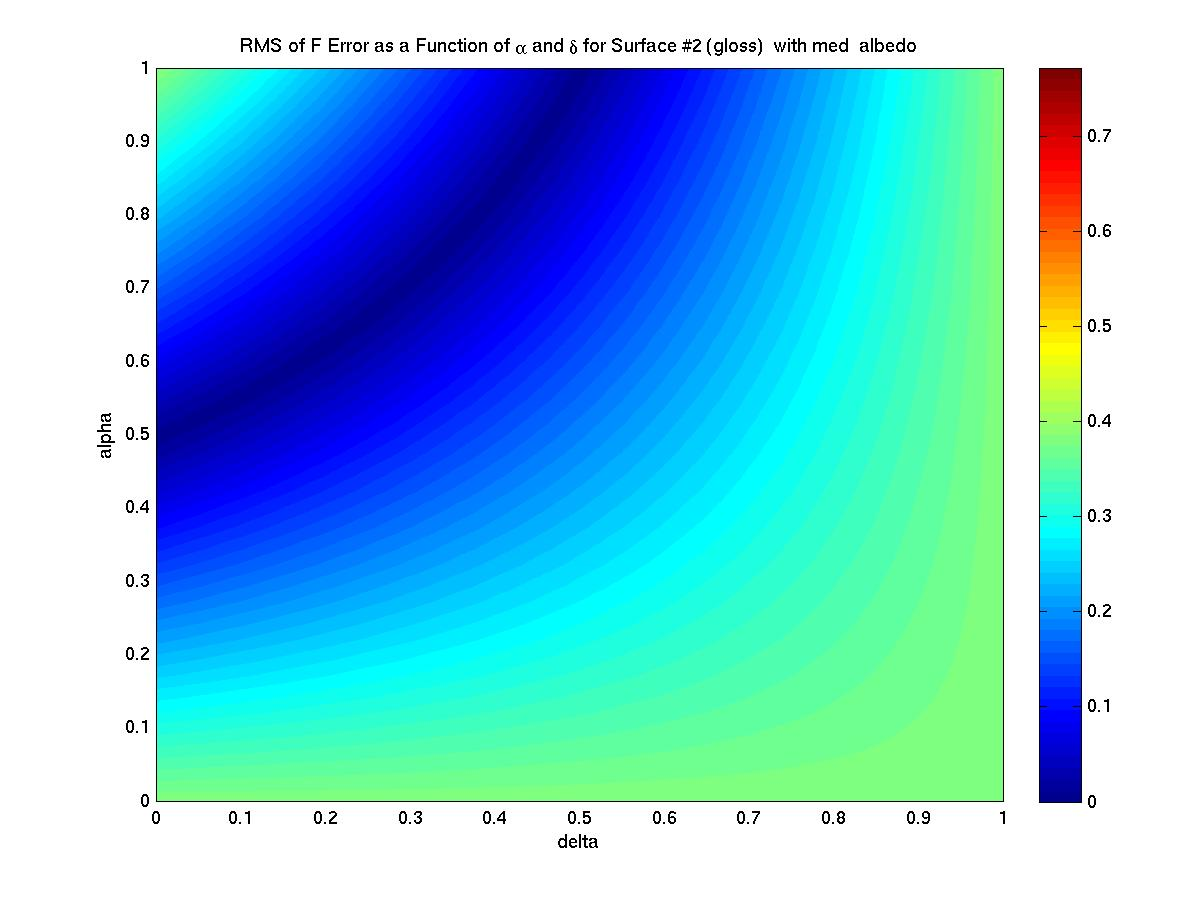
\includegraphics[width=65mm]{figs/sda/F_error_albedo__med_surf__gloss.jpg}
    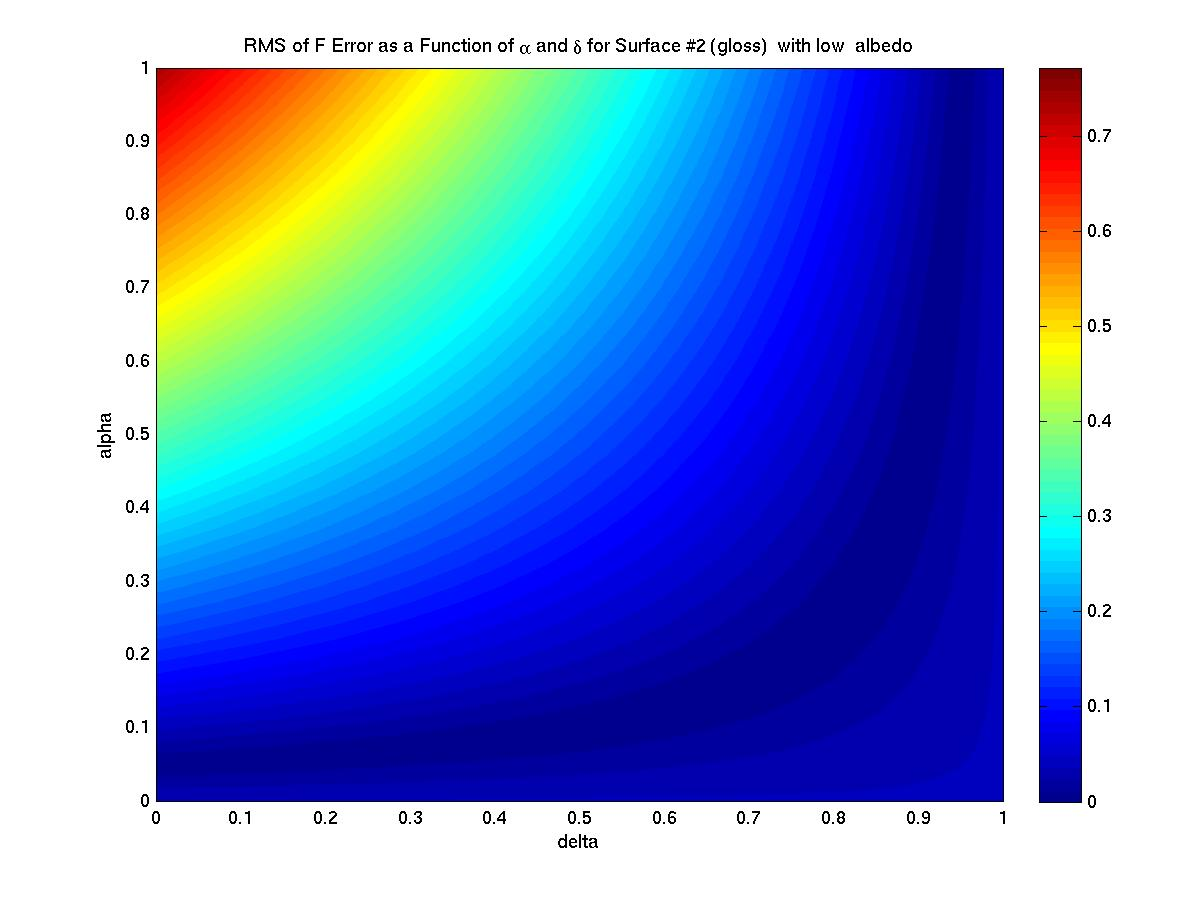
\includegraphics[width=65mm]{figs/sda/F_error_albedo__low_surf__gloss.jpg}
    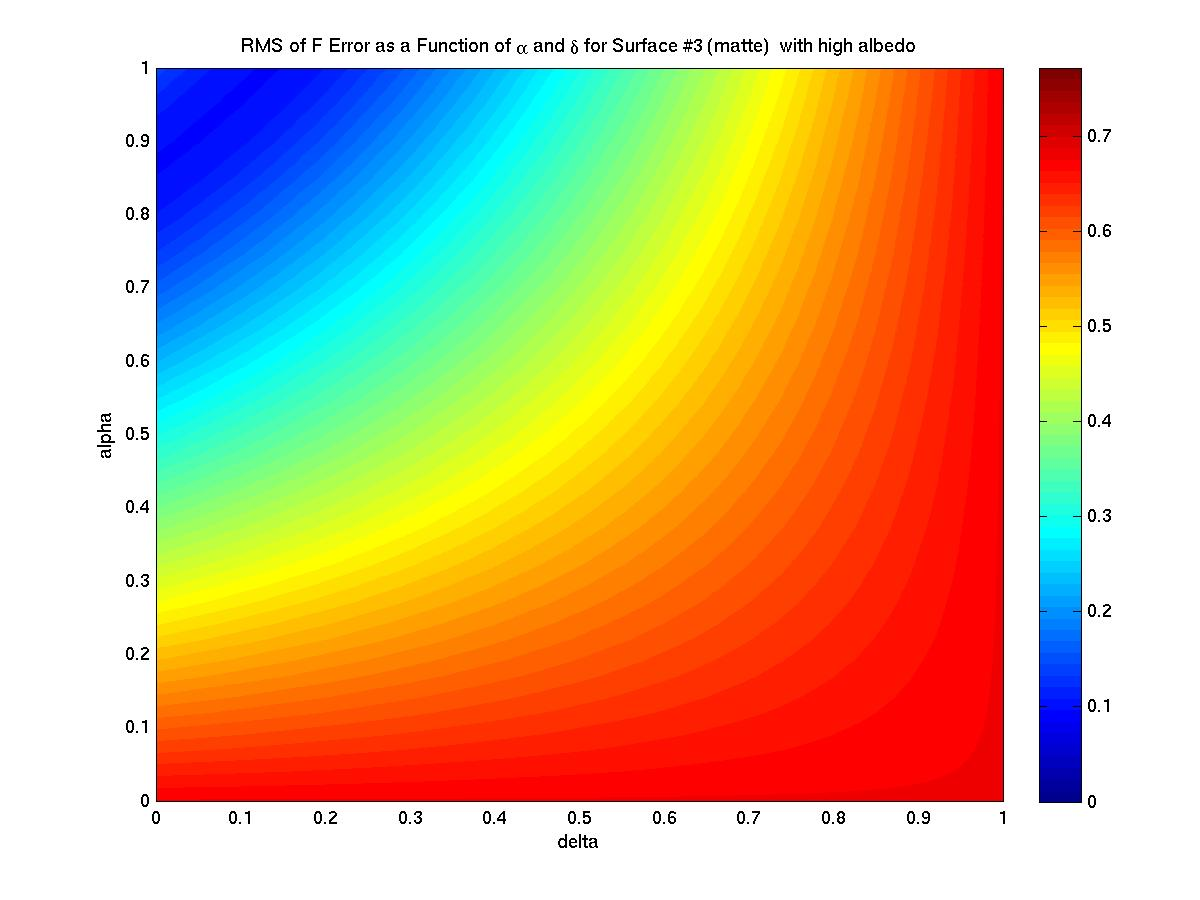
\includegraphics[width=65mm]{figs/sda/F_error_albedo_high_surf__matte.jpg}
    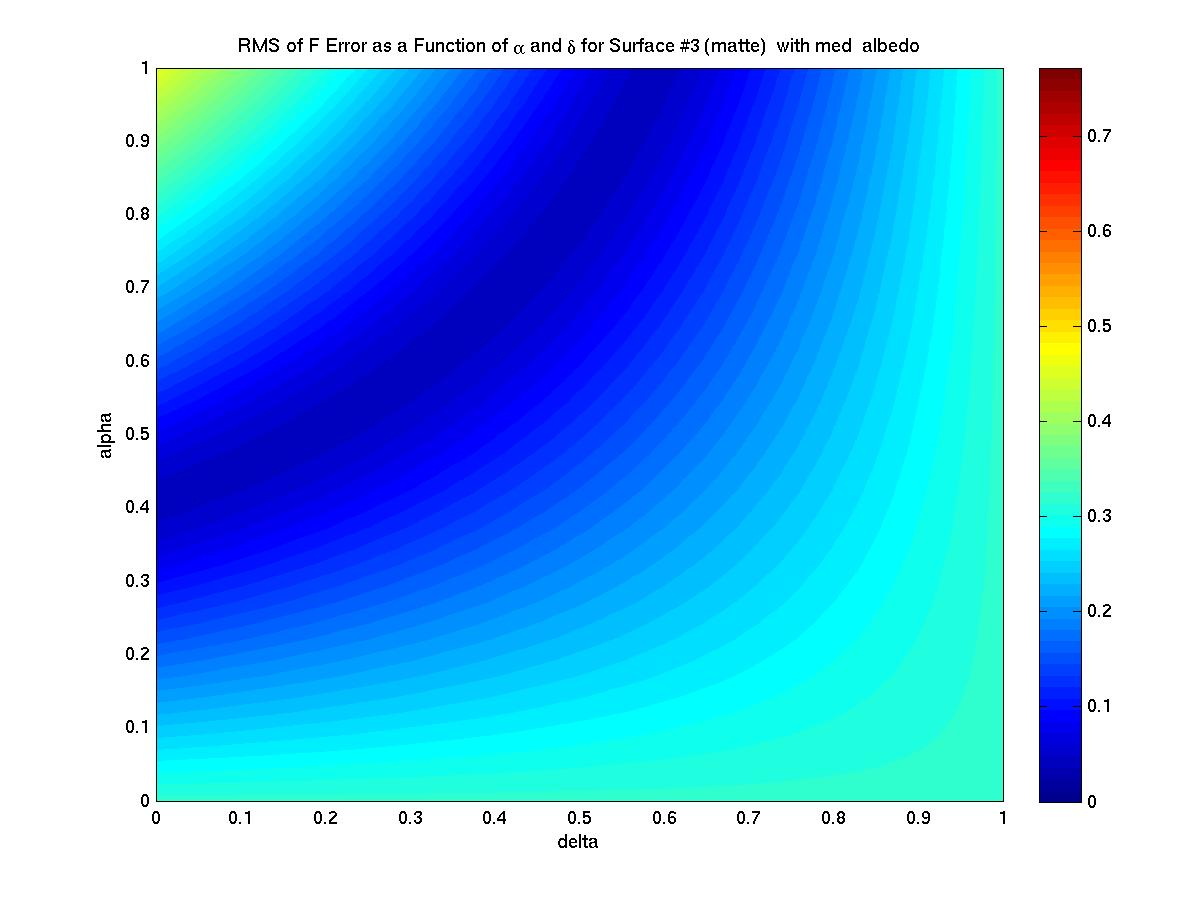
\includegraphics[width=65mm]{figs/sda/F_error_albedo__med_surf__matte.jpg}
    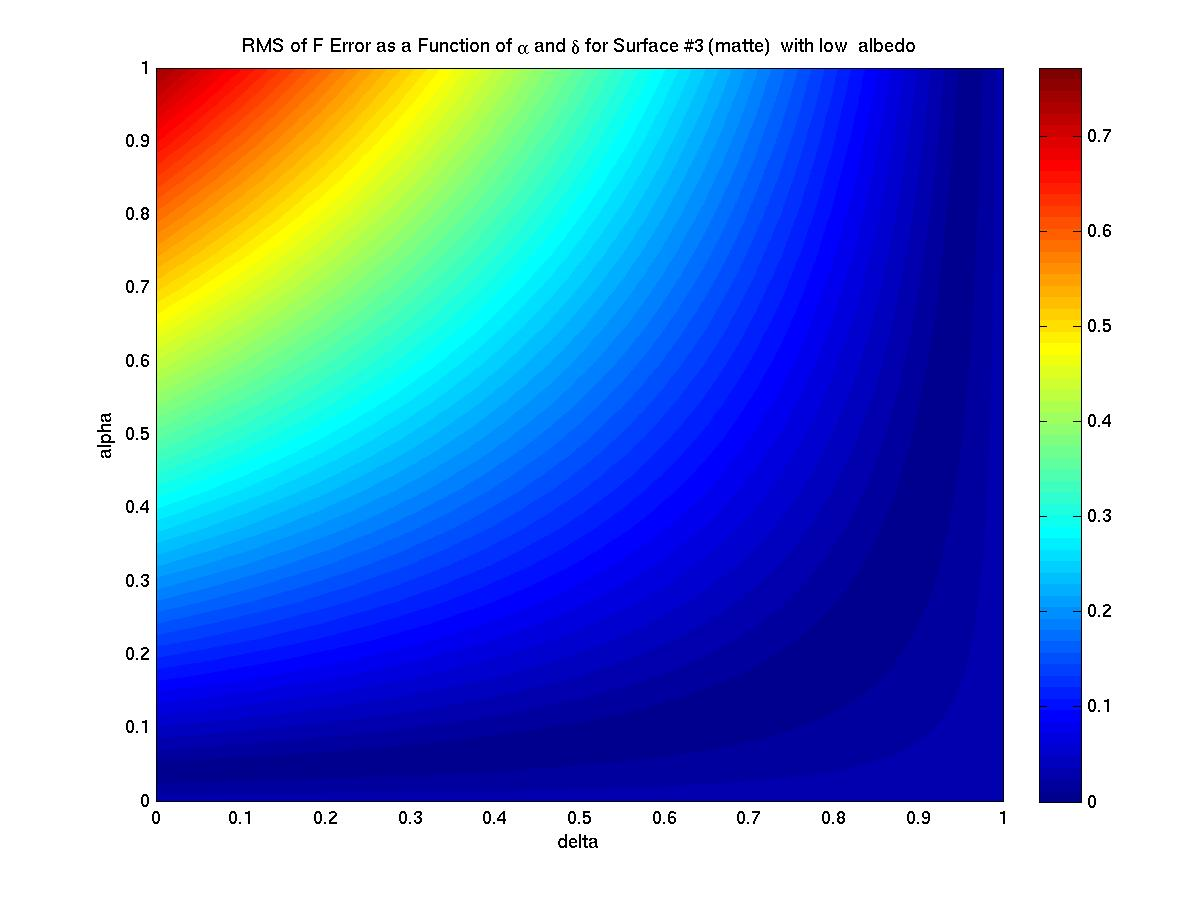
\includegraphics[width=65mm]{figs/sda/F_error_albedo__low_surf__matte.jpg}
    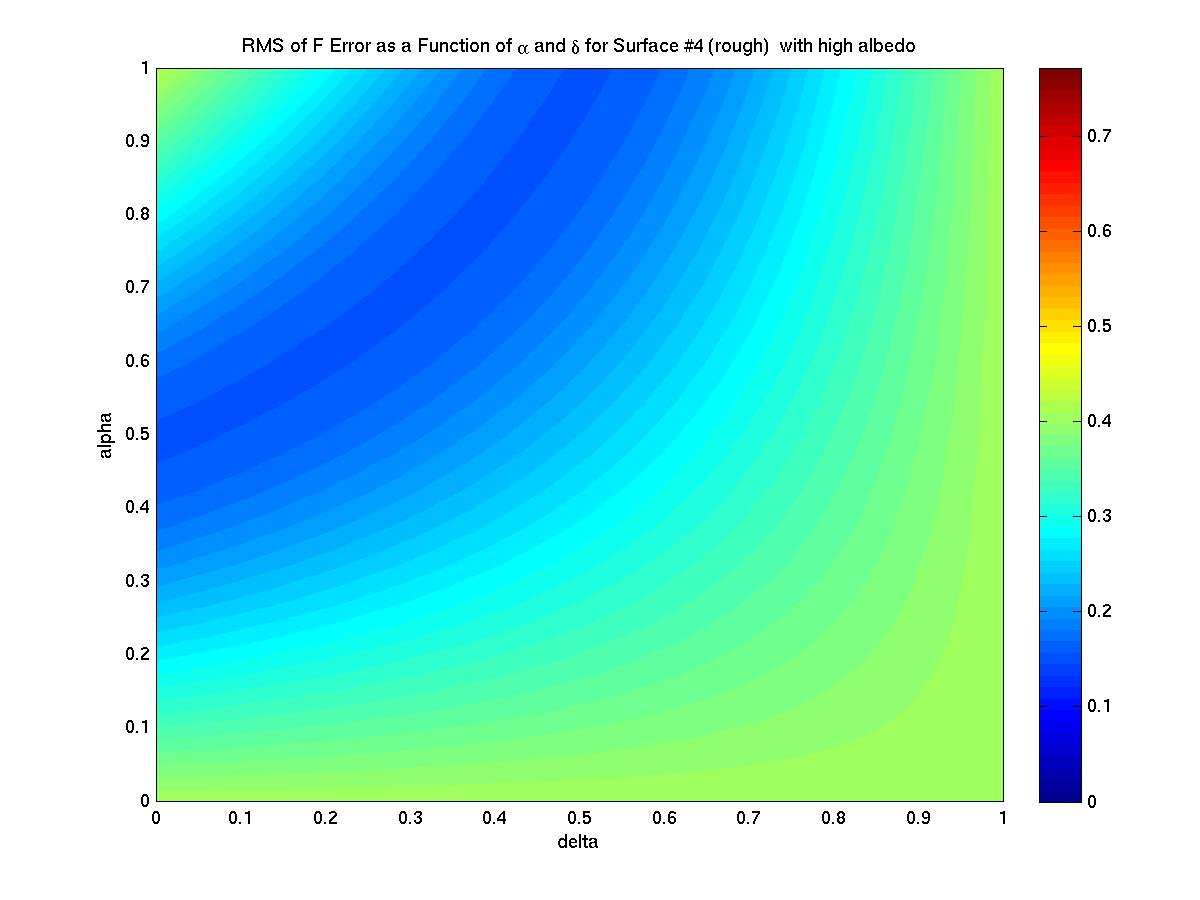
\includegraphics[width=65mm]{figs/sda/F_error_albedo_high_surf__rough.jpg}
    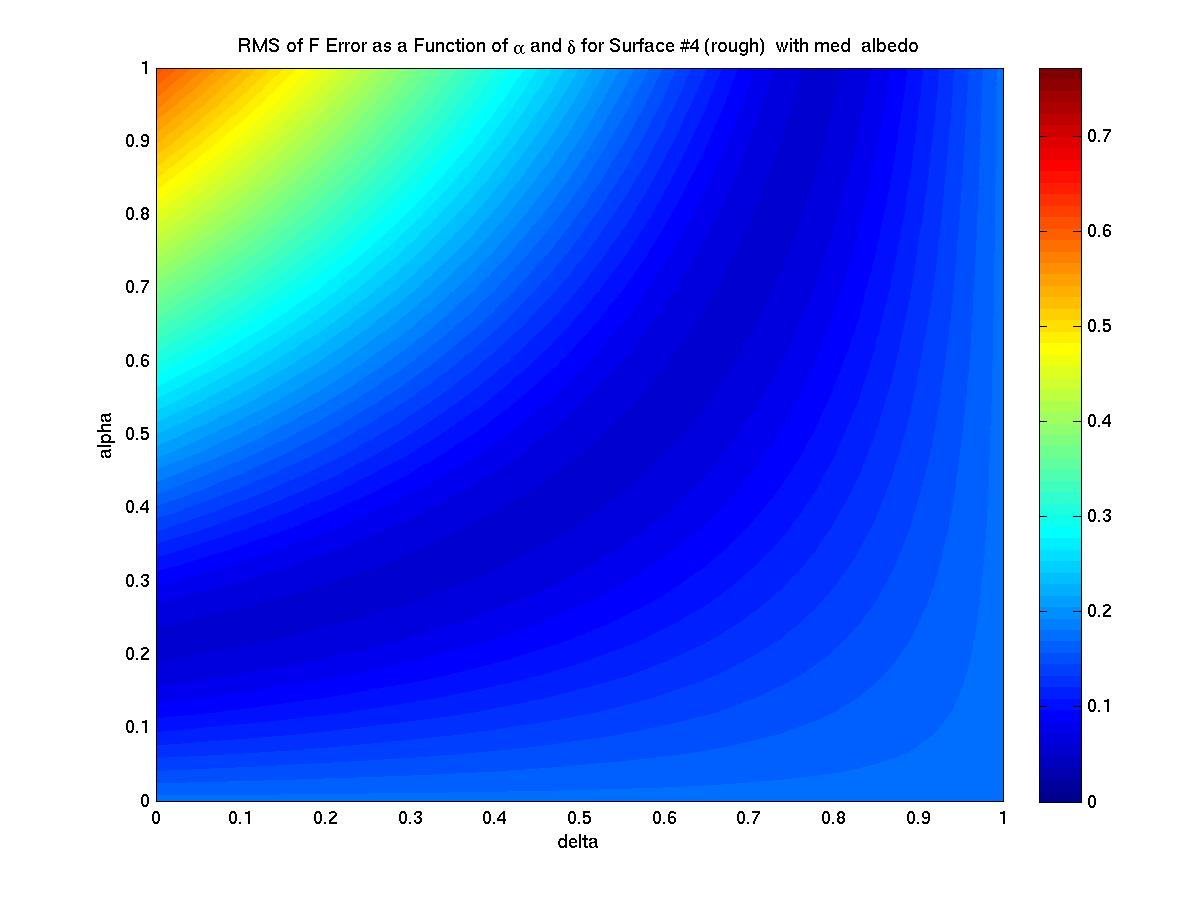
\includegraphics[width=65mm]{figs/sda/F_error_albedo__med_surf__rough.jpg}
    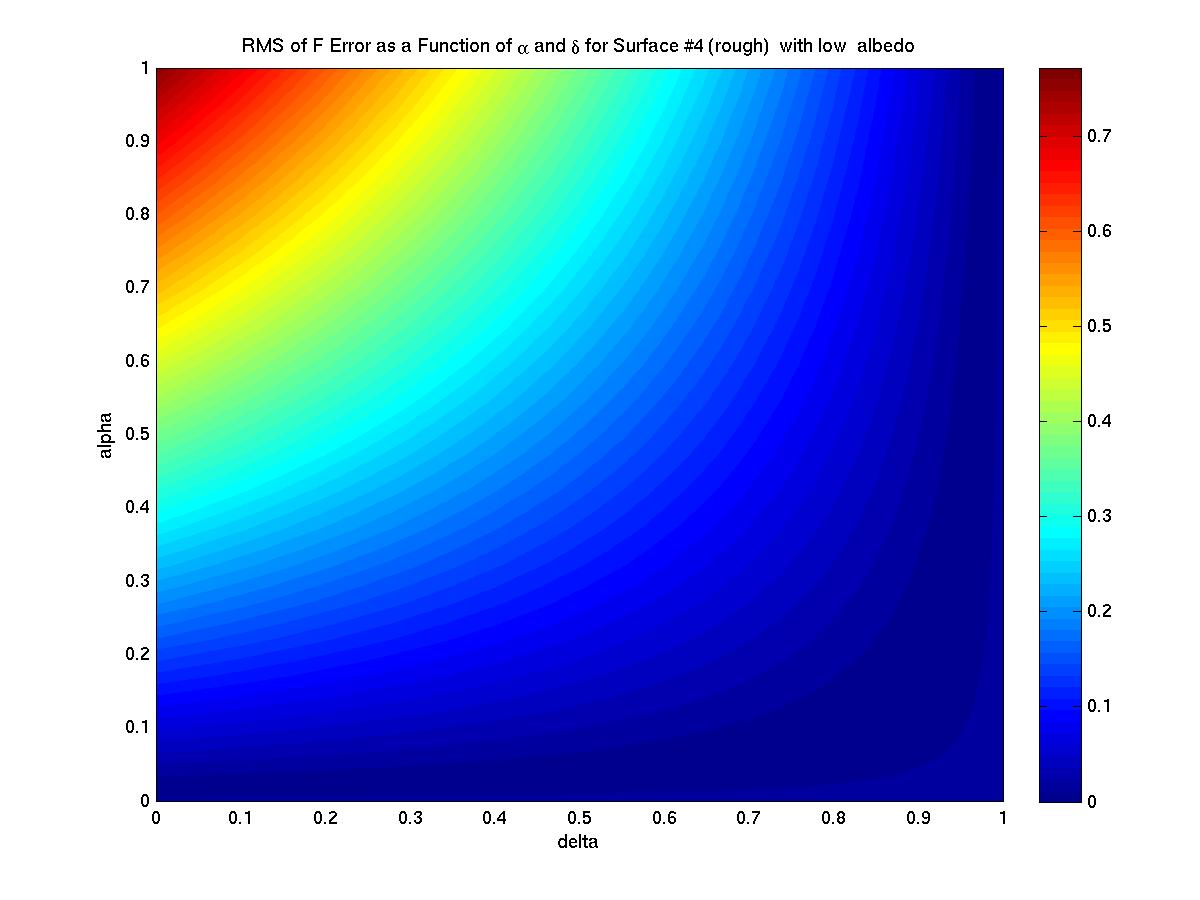
\includegraphics[width=65mm]{figs/sda/F_error_albedo__low_surf__rough.jpg}
  \end{minipage}
    \caption{Differences in the value of the magnitude of the model force, comparing the numerical simulation
    to the simplified model, as a function of $\alpha$ and $\delta$,
    presented in matrix formation with rows representing (from top) surface
    1-4, and columns representing (from left) high to low albedo.}
    \label{fig:ivv_sda_alpha_delta_F}
  \end{figure}

  \begin{figure}[!ht]
  \leftskip=-20mm
  \begin{minipage}[t]{200mm}\centering
    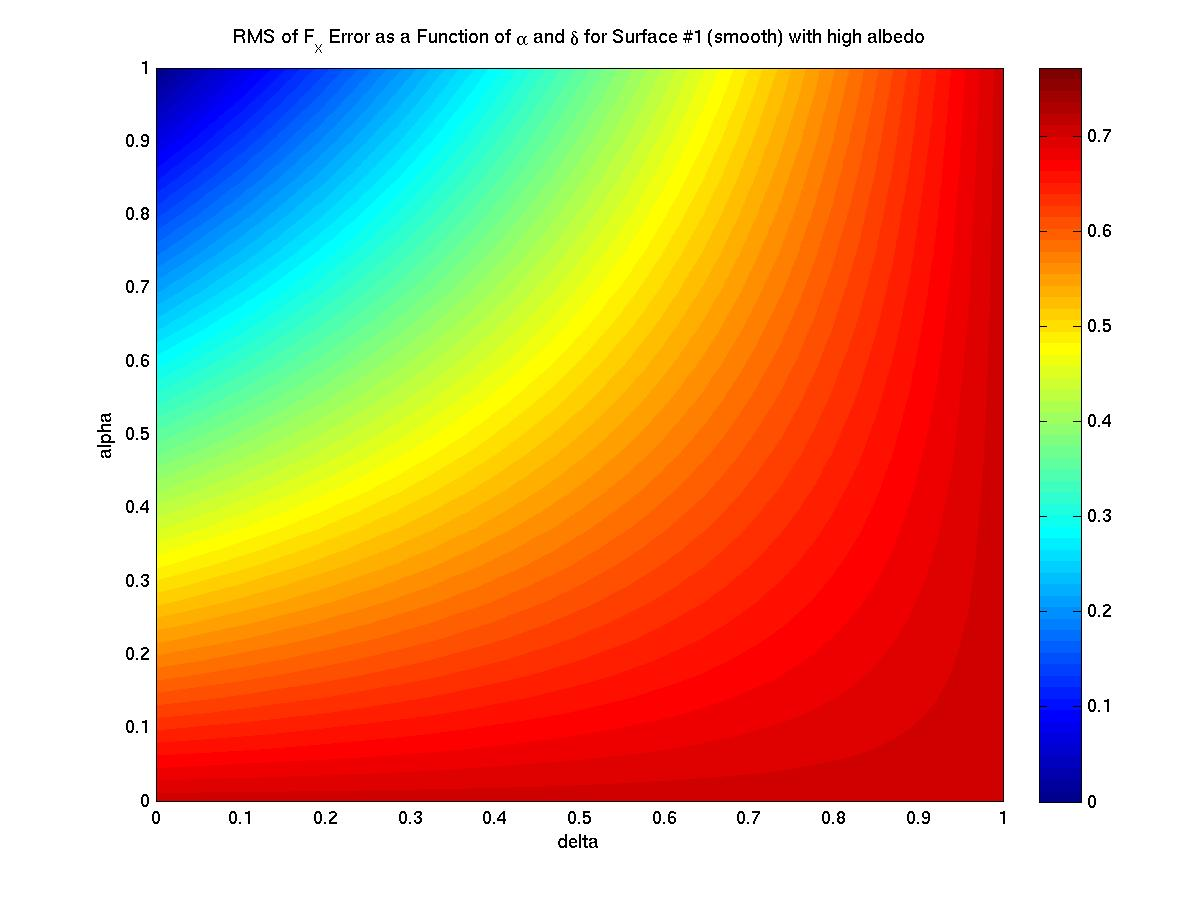
\includegraphics[width=65mm]{figs/sda/F_x_error_albedo_high_surf_smooth.jpg}
    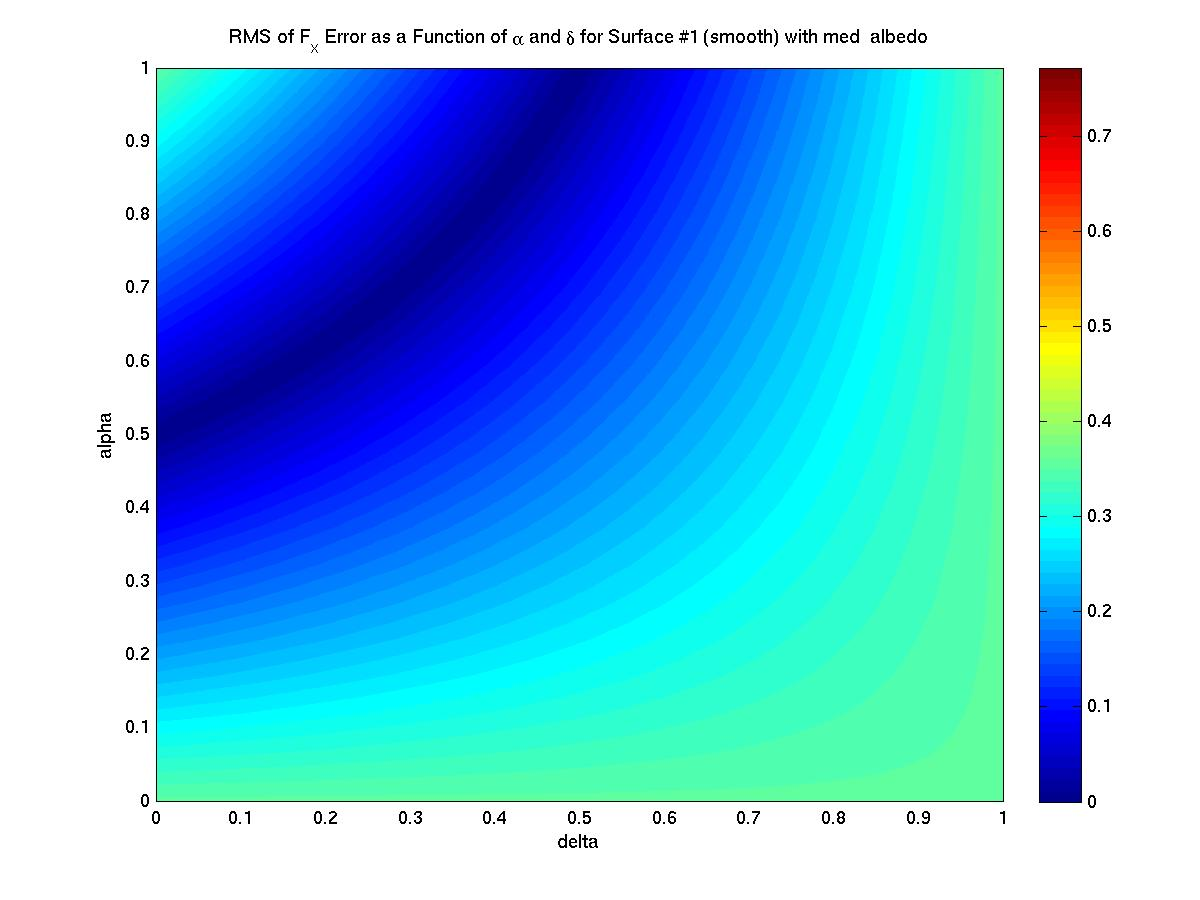
\includegraphics[width=65mm]{figs/sda/F_x_error_albedo__med_surf_smooth.jpg}
    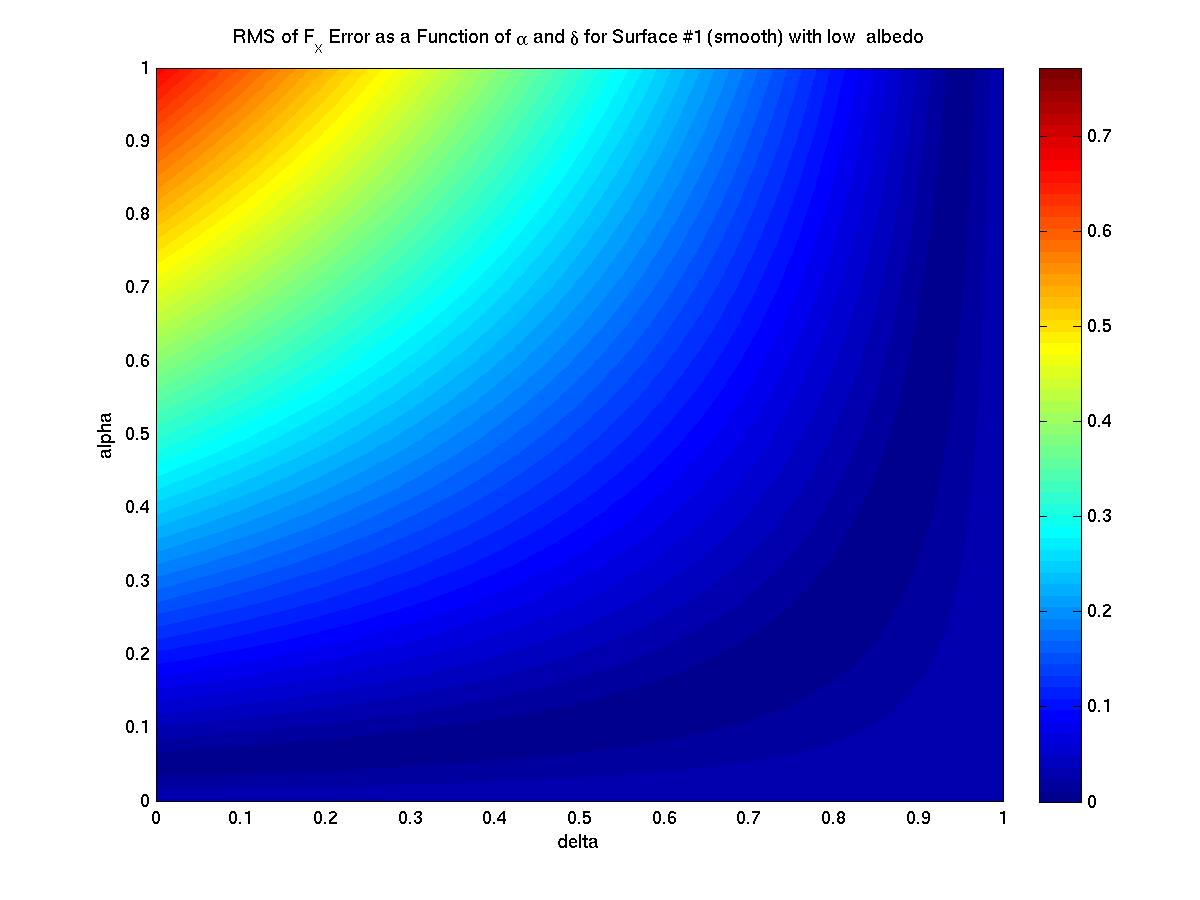
\includegraphics[width=65mm]{figs/sda/F_x_error_albedo__low_surf_smooth.jpg}
    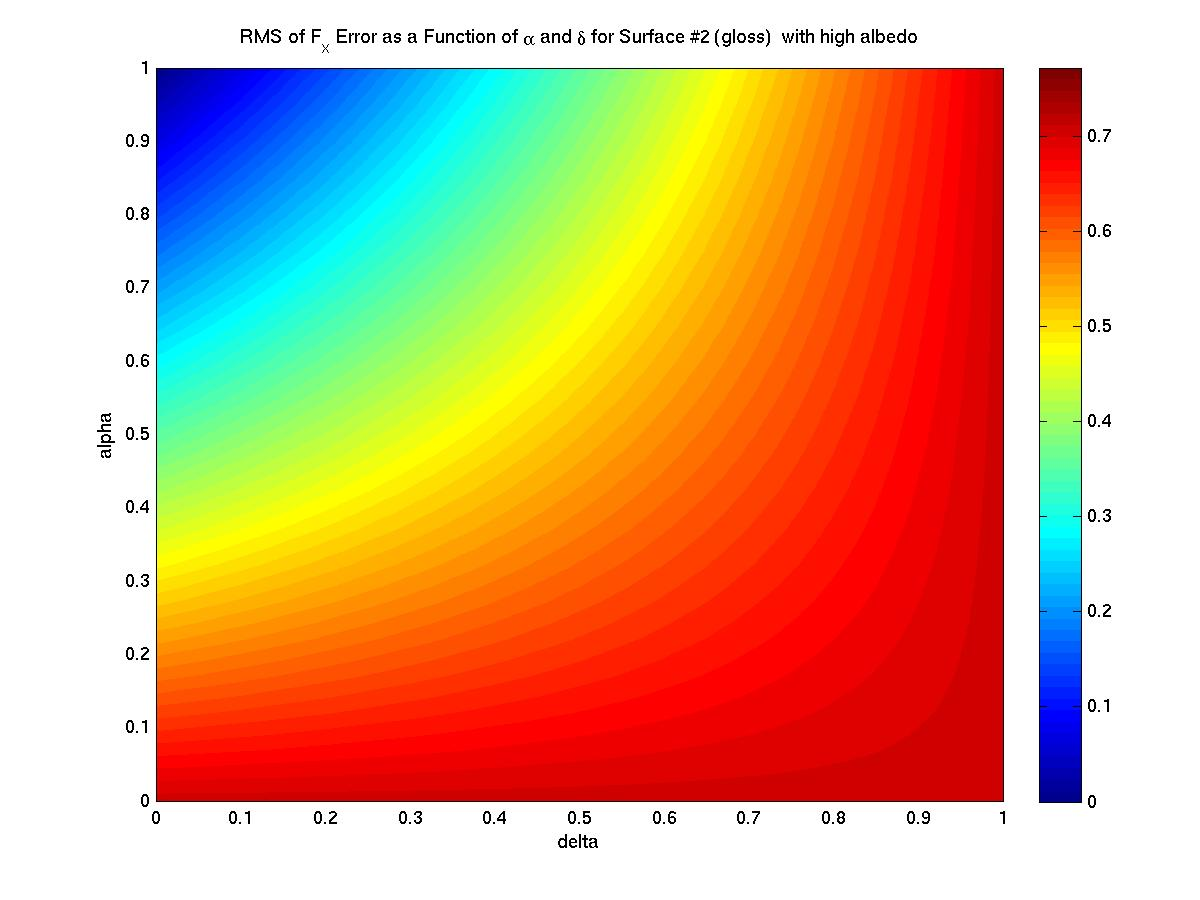
\includegraphics[width=65mm]{figs/sda/F_x_error_albedo_high_surf__gloss.jpg}
    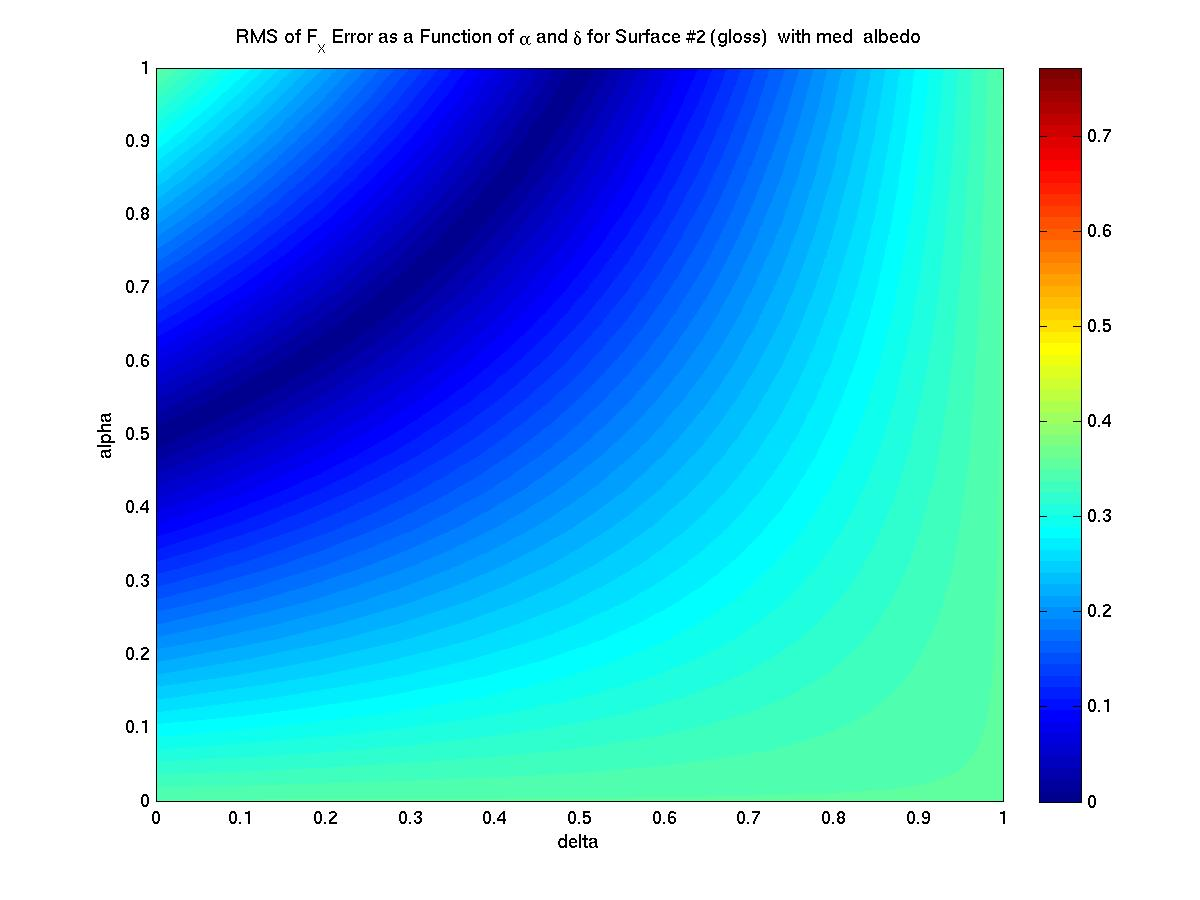
\includegraphics[width=65mm]{figs/sda/F_x_error_albedo__med_surf__gloss.jpg}
    \includegraphics[width=65mm]{figs/sda/F_x_error_albedo__low_surf__gloss.jpg}
    \includegraphics[width=65mm]{figs/sda/F_x_error_albedo_high_surf__matte.jpg}
    \includegraphics[width=65mm]{figs/sda/F_x_error_albedo__med_surf__matte.jpg}
    \includegraphics[width=65mm]{figs/sda/F_x_error_albedo__low_surf__matte.jpg}
    \includegraphics[width=65mm]{figs/sda/F_x_error_albedo_high_surf__rough.jpg}
    \includegraphics[width=65mm]{figs/sda/F_x_error_albedo__med_surf__rough.jpg}
    \includegraphics[width=65mm]{figs/sda/F_x_error_albedo__low_surf__rough.jpg}
  \end{minipage}
    \caption{Differences in the value of the x-component of the model force, comparing the
    numerical simulation to
    the simplified model, as a function of $\alpha$ and $\delta$,
    presented in matrix formation with rows representing (from top) surface
    1-4, and columns representing (from left) high to low albedo.}
    \label{fig:ivv_sda_alpha_delta_Fx}
  \end{figure}
  \begin{figure}[!ht]
  \leftskip=-20mm
  \begin{minipage}[t]{200mm}\centering
    \includegraphics[width=65mm]{figs/sda/F_z_error_albedo_high_surf_smooth.jpg}
    \includegraphics[width=65mm]{figs/sda/F_z_error_albedo__med_surf_smooth.jpg}
    \includegraphics[width=65mm]{figs/sda/F_z_error_albedo__low_surf_smooth.jpg}
    \includegraphics[width=65mm]{figs/sda/F_z_error_albedo_high_surf__gloss.jpg}
    \includegraphics[width=65mm]{figs/sda/F_z_error_albedo__med_surf__gloss.jpg}
    \includegraphics[width=65mm]{figs/sda/F_z_error_albedo__low_surf__gloss.jpg}
    \includegraphics[width=65mm]{figs/sda/F_z_error_albedo_high_surf__matte.jpg}
    \includegraphics[width=65mm]{figs/sda/F_z_error_albedo__med_surf__matte.jpg}
    \includegraphics[width=65mm]{figs/sda/F_z_error_albedo__low_surf__matte.jpg}
    \includegraphics[width=65mm]{figs/sda/F_z_error_albedo_high_surf__rough.jpg}
    \includegraphics[width=65mm]{figs/sda/F_z_error_albedo__med_surf__rough.jpg}
    \includegraphics[width=65mm]{figs/sda/F_z_error_albedo__low_surf__rough.jpg}
  \end{minipage}
    \caption{Differences in the value of the z-component of the model force, comparing the
    numerical simulation to
    the simplified model, as a function of $\alpha$ and $\delta$,
    presented in matrix formation with rows representing (from top) surface
    1-4, and columns representing (from left) high to low albedo.}
    \label{fig:ivv_sda_alpha_delta_Fz}
  \end{figure}
      Of interest, there is a trend that as the surface gets rougher, $\alpha
      $ gets smaller and/or  $\delta $ gets larger.  This is expected behavior; as the surface gets rougher, more photons will be reflected ``down'' into the surface and be absorbed, reducing the albedo, those photons that are reflected upward are going to be more scattered, appearing as diffuse reflection more than specular reflection.
      For all four surfaces, the albedo settings (low, med, or
      high) are assigned by the value of the albedo of each
      microscopic plate.

  \end{description}

  \clearpage

\subsection{Validation of the Plate Model Assumptions}
\label{sec:platemodelvalid}
\test{Validation of the Plate Model Assumptions}
  \label{test:plate_model}
  \begin{description}
   \item{Purpose:}\newline
    To validate that, for the purposes of radiation
    pressure calculations, curved surfaces can be
    approximated by crude, gross-feature-only, flat plate
    models, and to assess the degree to which doing so
    introduces error into the system.

   \item{Procedure:}\newline
    The response of a square cuboid --- of side \it s \rm and length \it L
    \rm --- to a radiation field is compared
    to that of a cylinder of comparable dimensions, with the
    cuboid representing the flat-plate approximation to the
    cylinder.  The two objects were rotated in a constant radiation
    field with the long-axis perpendicular to the flux vector, as shown in
    figure~\ref{fig:ivv_isotherm_fig1}.

    This test was conducted using the \JEODid\ algorithms ported into MATLAB, while test \vref{test:sim4} compares the difference directly between the spherical default surface, and a cubic flat-plate surface.

    \begin{figure}[!ht]
      \begin{center}
      \includegraphics[width=150mm]{figs/isoth_app/iso_app_figs1.jpg}
      \end{center}
      \caption{Orientation of the cylinder and cuboid.}
      \label{fig:ivv_isotherm_fig1}
    \end{figure}

    The effects from the ends of the objects were ignored, which is
    essentially equivalent to assuming the objects to be long and thin.
    Rotation angles
    are measured counterclockwise from the lowest point on the
    object, as shown in figure~\ref{fig:ivv_isotherm_fig4}.

    \begin{figure}[!ht]
      \begin{center}
      \includegraphics[width=70mm]{figs/isoth_app/iso_app_figs4.jpg}
      \end{center}
      \caption{Definition of angle $\theta$.}
      \label{fig:ivv_isotherm_fig4}
    \end{figure}

    The cuboid starts `sitting' on one face, as shown
    in figure~\ref{fig:ivv_plate_model_fig1}.
    \begin{figure}[!ht]
      \begin{center}
      \includegraphics[width=90mm]{figs/cyl_cub_comp/cyl_cub_fig1.jpg}
      \end{center}
      \caption{Orientation of the cylinder and cuboid.}
      \label{fig:ivv_plate_model_fig1}
    \end{figure}

    The two objects were configured to allow for two extremes of temperature
    structures:
    \begin{enumerate}
     \item{}The temperature was uniform across the object (isothermal
     approximation).
     \item{}The temperature was spatially variable, with plates assumed to be
       thermally isolated for maximum temperature differential.  For this, the
       cylinder was configured to comprise a large collection of thin strips,
       running the length of the cylinder.
    \end{enumerate}

    Data are taken from the steady states of the two objects for
    each configuration (i.e. after initial transients have died away, the variability is due entirely to the rotation, and the temperature -- and therefore the force -- associated with each plate can be expressed as a function of $\theta$ only, with no other dependency on time).

    Finally, the dimensions of the cuboid were adjusted to investigate whether
    it was more important to have equivalent surface area, or equivalent
    enclosed volume as an approximation to the cylinder.

   \item{Mathematical development} \ \newline
     This section develops the equations used in these tests.

     \begin{enumerate}
     \item{Cuboid}
       \begin{enumerate}
         \item{Absorption:}\ \newline
           The rate at which energy is absorbed is the product of the flux
           vector, the projected area, and the absorptivity (equal to 1-albedo).
           The force, or momentum flux, is related to the energy flux by the
           speed of light.  The
           absorption will only produce a force in the direction of the incident
           radiation.  It will not be a constant, as the cuboid projects
           different cross section as it rotates.
           \begin{figure}[!ht]
             \begin{center}
             \includegraphics[width=90mm]{figs/isoth_app/iso_app_figs3.jpg}
             \end{center}
             \caption{The surface area projected perpendicular to the
                illumination vector.}
             \label{fig:ivv_isotherm_fig3}
           \end{figure}

           Incident flux falls on two projected areas, one of area
           $sL\sin \theta $ , and another of area $sL\cos \theta $ ,

           \begin{equation}
             \vec {F} = \left( \frac {1-\alpha}{c} \right)
             \phi s L (\sin \theta + \cos \theta) \hat {i}
           \end{equation}
          \item{Specular Reflection:}\ \newline
            Incident flux falls on the same two surfaces, where some fraction
            $\alpha $ is reflected, ($\alpha(1-\delta)$ is reflected
            specularly).  There are two force ``components'', one from
            `stopping' the incident radiation (in direction of radiation
            vector), and one `recoiling' from the reflected radiation (in
            direction opposite the radiation vector).  Use $\hat{r}_{i}$ to
            represent the direction of (specularly) reflected radiation from
            surface~\textit{i}.

            \begin{equation*}
            \vec {F}=\frac{\alpha (1-\delta)}{c} \phi sL \left(\sin \theta
            (\hat{i}-\hat{r}_{1})+\cos \theta (\hat{i}-\hat{r}_{2})\right)
            \end{equation*}


            \begin{figure}[!ht]
            \begin{center}
              \includegraphics[width=100mm]{figs/isoth_app/iso_app_figs5.jpg}
              \caption{Schematic of the reflection from the two illuminated
                 sides.}
              \label{fig:ivv_isotherm_fig5}
            \end{center}
            \end{figure}

Figure~\ref{fig:ivv_isotherm_fig5} illustrates that by geometry,
            $\hat {r}_{1} = - \hat {r}_{2}$, and that
            $\hat {r}_{1} = \cos 2\theta \hat {i} + \sin 2 \theta \hat {j}$.

            Hence,
            \begin{equation*}
            \vec {F}=\frac{\alpha (1-\delta)}{c}\phi sL
            \left[\hat{i}\left(\sin \theta +\cos \theta +\cos 2\theta
            \left(\cos \theta -\sin \theta \right)\right)+
            \hat{j} \left( \sin 2 \theta
            \left(\cos \theta -\sin \theta \right)\right) \right]
            \end{equation*}

            Simplifying,

            \begin{equation}
              \vec {F}=\frac{\alpha (1-\delta)}{c}\phi sL \left[
              \hat{i}2\left(\sin^{3} \theta +\cos^3 \theta \right)+
              \hat{j}\left(\sin 2\theta \left(\cos \theta -\sin \theta
              \right)\right) \right]
            \end{equation}

           \item{Diffuse Reflection:}\ \newline
            The same two sides again involved, this time

            \begin{equation*}
            \vec {F}=\frac{\alpha \delta}{c}\phi sL
            \left[
              \sin \theta
              \left(
                \hat {i} + \frac{2}{3}
                \left(
                  \sin \theta \hat {i} - \cos \theta \hat {j}
                \right)
              \right)
              + \cos \theta
              \left(
                \hat {i} + \frac{2}{3}
                \left(
                  \cos \theta \hat {i} + \sin \theta \hat {j}
                \right)
              \right)
            \right]
            \end{equation*}

            which simplifies to
            \begin{equation}
              \vec {F}=\frac{\alpha \delta}{c}\phi sL \left( \sin \theta +
              \cos \theta + \frac{2}{3} \right) \hat {i}
            \end{equation}

          \item{Emission:}\ \newline
            The cuboid comprises four sides, all of which emit.
            \begin{enumerate}
            \item{Non-isothermal case:}\ \newline
            Each side will emit differently, because each side will have an
            independent temperature.  As a side rotates into illumination, it
            will pass through a minimum temperature, and reach a maximum
            temperature shortly before passing back into shadow, as shown in
            Figure~\ref{fig:ivv_isotherm_fig2}.
            In order to calculate the force as a function of
            angle, first the temperature must be known as a function of angle.
            In this test, that is completed by numerical integration.

            \begin{figure}[!ht]
             \begin{center}
             \includegraphics[width=50mm]{figs/isoth_app/iso_app_figs2.jpg}
             \end{center}
             \caption{The temperature variation across the non-isothermal
               cuboid.}
             \label{fig:ivv_isotherm_fig2}
           \end{figure}


            Consider an arbitrary plate, call it plate\#1:

            The rate at which the temperature changes is
            given by:

            \begin{equation*}
              \frac{dT}{dt} =
              \begin{cases}
                \frac{4sL}{C} \left((1-\alpha) \phi \sin
                \theta - \epsilon \sigma T^{4} \right) & illuminated \\
                -\frac{4sL}{C} \epsilon \sigma T^{4}  & shaded
              \end{cases}
             \end{equation*}

            where $C$ is the heat capacity of the entire cuboid (hence the heat
            capacity of one ``side'' is C/4).

            The emissive force acting on the plate is:

            \begin{equation*}
						\vec {F}(\theta) = \frac{2}{3} \frac{1}{c} \frac{dE}{dT} \vec \hat
						{n} = \frac {2sL \epsilon \sigma T(\theta)^{4}}{3c}
            \left(\sin \theta \hat {i} - \cos \theta \hat {j} \right)
            \end{equation*}

            Each of the other plates, $i=2,3,4$, can be considered as having
            rotated through an additional angle of $\pi (i-1) /2$ and the overall force
            obtained from the summation over the four plates, with
            $\theta_{i}=\theta + \pi (i-1) /2$.

            \begin{equation}
              \vec F(\theta) = \frac {2sL \epsilon \sigma}{3c} \sum_{i=1}^4
                T(\theta_i)^4 \left(\sin \theta_i \hat {i} - \cos \theta_i \hat
                 {j} \right)
            \end{equation}
            \item{Isothermal case:} \ \newline
            Each side will emit at the same rate, and the emissive forces will
            cancel to zero.
            Because the emitting area is constant, but the receiving area is
            variable, the temperature varies in time.

            \begin{equation}
            \frac{dT}{dt} = \frac{sL}{C} \left(
              (1-\alpha) \phi \left(
                \vert \sin \theta \vert + \vert \cos \theta \vert \right)
              - 4 \epsilon \sigma T^{4} \right)
            \end{equation}
            \end{enumerate}
        \end{enumerate}

      \item {Cylinder}
        \begin{enumerate}
           \item{Absorption:}\ \newline
            The rate at which energy is absorbed is the product of the flux
            vector, the projected area, and the absorptivity (1-albedo).  The
            force is related to the energy rate by the speed of light.
            \begin{equation}
              \vec {F} = \frac {1-\alpha}{c} 2 R L \phi \hat {i}
            \end{equation}
          \item{Specular reflection:}\ \newline
            Similar to the case for the cuboid, there are two considerations
            to the force, one from `stopping' the incident radiation (in
            direction of radiation vector), and one `recoiling' from the
            reflected radiation (in direction opposite the radiation vector).
            Consider a thin strip of the cylinder, of length L subtending an
            angle $d \theta$ located at rotation angle $\theta$.

            \begin{equation*}
            \vec {F}=\frac{\alpha (1-\delta)}{c}\phi RL d \theta
            \left[\hat{i}\left(\sin \theta - \cos 2\theta \sin \theta \right)
            - \hat{j} \left(\sin 2\theta \sin \theta \right) \right]
            \end{equation*}

            Such strips will contribute to the force as long as
            $0 \leqslant \theta \leqslant \pi$.  Integrating produces

            \begin{equation}
              \vec {F}=\frac{8 \alpha (1-\delta)}{3 c}\phi RL \hat {i}
            \end{equation}
          \item{Diffuse Reflection:}\ \newline
            Using a similar analysis based on the development for the cuboid
            and integrating again yields

            \begin{equation}
              \vec {F}=\frac{ \alpha \delta}{c}\phi RL \left( 2+ \frac{\pi}{3}
              \right) \hat {i}
            \end{equation}
          \item{Emission:}\ \newline
           \begin{enumerate}
           \item{Non-isothermal case:}\ \newline
            The cylinder comprises $\frac{2 \pi}{d \theta}$ sides, compared to
            the cuboid's four.  Similar to the cuboid, each side will have an
            independent temperature.  In order to calculate the force as a
            function of angle, first the temperature must be known as a function
            of angle.

            Consider an elemental strip: The rate at which the
            temperature changes is given by:

             \begin{equation*}
              \frac{dT}{dt} =
              \begin{cases}
                \frac{2RL \pi}{C} \left((1-\alpha) \phi \sin
                \theta - \epsilon \sigma T^{4} \right) & illuminated \\
                -\frac{2RL \pi}{C} \epsilon \sigma T^{4}  & shaded
              \end{cases}
            \end{equation*}

            where $C$ is the heat capacity of the entire cylinder.

						The force acting on an element is:

            \begin{equation}
              \vec {dF}(\theta) = \frac {2R d\theta L \epsilon \sigma \left(
              T(\theta) \right) ^{4}}{3c} \left(\sin \theta \hat {i} -
              \cos \theta \hat {j} \right)
            \end{equation}

            which can be integrated numerically over the entire cylinder once
            the steady state temperature structure is known.

           \item{Isothermal case:}\ \newline
            The net force from emission for an isothermal cylinder is zero, by
            symmetry.   Also by symmetry, there is no temporal temperature
            variation.
           \end{enumerate}
        \end{enumerate}
      \end{enumerate}

   \item{Results:}

     Data were collected for cases of low, medium, and high values of albedo,
     for cases of
     low, medium and high values for the heat capacity (essentially, this
     affects only the temperature response to the absorbed radiation; this
     variation is equivalent to varying the rotational period), and for the
     cases of totally diffuse and totally specular reflection.

     The x-component of the force is larger than the y-component in all cases.

     The dominant features, shown  in
     Figures~\ref{fig:ivv_platemod_fig1}~to~\ref{fig:ivv_platemod_fig4}
     are that the forces due to radiation are:
     \begin{itemize}
        \item{}Strongly affected by the extent to which the plate
          temperature varies.
        \item{}Weakly affected by the approximation of the flat-plate model to the curved
           surface.
      \end{itemize}

      Figure~\ref{fig:ivv_platemod_impulse} shows the integration of the
      force over time, or the total impulse applied to the surface as a function of time; this is particularly useful because it smooths out the
      fluctuations that result from the flat-plate approximation to the smooth
      surface, and allows a comparison to be made of the average force applied.
      From
      figures~\ref{fig:ivv_platemod_fig1}~to~\ref{fig:ivv_platemod_fig4}
      it is clear that
      the variation with time of the force on the cuboid depends strongly on
      the values used to represent:
      \begin{enumerate}
        \item{}The albedo
        \item{}The relative strength of the specular to diffuse reflection
        \item{}The extent to which the temperature varies.
      \end{enumerate}

      Conversely, the cylinder shows no time variation
      regardless of variations in those values.
      However, the analysis leading to
      Figure~\ref{fig:ivv_platemod_impulse}
      demonstrates that, providing that the size is handled appropriately, the
      time-integrated difference between the cylinder and cuboid is
      negligible, and hence it can be concluded that the cuboid is a reasonable
      approximation to the cylinder across a range of values for the albedo,
      the temperature fluctuations.  Furthermore, Figure~\ref{fig:ivv_platemod_specdiff} demonstrates that the difference between specular and diffuse reflection, averaged over time, are also not very significant.

      Finally, figure~\ref{fig:ivv_platemod_size} contrasts two sizes for
      the cuboid.  It can safely be concluded that it is more important to
      conserve the surface area of the approximated vehicle than to conserve the
      enclosed volume of the approximated vehicle.  Data presented in
      Figures~\ref{fig:ivv_platemod_fig1}~to~\ref{fig:ivv_platemod_specdiff}
      have the cylinder and cuboid with equal surface area.

     \begin{figure}
       \includegraphics[width=160mm]{figs/Plate_mod/Fx_ref_spc_alb_high.jpg}
       \includegraphics[width=160mm]{figs/Plate_mod/Fx_ref_spc_alb_mid_.jpg}
       \includegraphics[width=160mm]{figs/Plate_mod/Fx_ref_spc_alb_low_.jpg}
       \caption{The x-component of force due to radiation with specular
       reflection.  Each chart represents a different albedo, and contains
       plots for different temperature-response models.  A model with low
       heat capacity will have a high temperature response.}
       \label{fig:ivv_platemod_fig1}
     \end{figure}
     \begin{figure}
       \includegraphics[width=160mm]{figs/Plate_mod/Fx_ref_dif_alb_high.jpg}
       \includegraphics[width=160mm]{figs/Plate_mod/Fx_ref_dif_alb_mid_.jpg}
       \includegraphics[width=160mm]{figs/Plate_mod/Fx_ref_dif_alb_low_.jpg}
       \caption{The x-component of force due to radiation with diffuse
       reflection.  Each chart represents a different albedo, and contains
       plots for different temperature-response models.  A model with low
       heat capacity will have a high temperature response.}
       \label{fig:ivv_platemod_fig2}
     \end{figure}
     \begin{figure}
       \includegraphics[width=160mm]{figs/Plate_mod/Fy_ref_spc_alb_high.jpg}
       \includegraphics[width=160mm]{figs/Plate_mod/Fy_ref_spc_alb_mid_.jpg}
       \includegraphics[width=160mm]{figs/Plate_mod/Fy_ref_spc_alb_low_.jpg}
       \caption{The y-component of force due to radiation with specular
       reflection.  Each chart represents a different albedo, and contains
       plots for different temperature-response models.  A model with low
       heat capacity will have a high temperature response.}
       \label{fig:ivv_platemod_fig3}
     \end{figure}
     \begin{figure}
       \includegraphics[width=160mm]{figs/Plate_mod/Fy_ref_dif_alb_high.jpg}
       \includegraphics[width=160mm]{figs/Plate_mod/Fy_ref_dif_alb_mid_.jpg}
       \includegraphics[width=160mm]{figs/Plate_mod/Fy_ref_dif_alb_low_.jpg}
       \caption{The y-component of force due to radiation with diffuse
       reflection.  Each chart represents a different albedo, and contains
       plots for different temperature-response models.  A model with low
       heat capacity will have a high temperature response.}
       \label{fig:ivv_platemod_fig4}
     \end{figure}

     \begin{figure}[!ht]
     \leftskip=-20mm
     \begin{minipage}[t]{200mm}\centering
     \includegraphics[width=65mm]{figs/Plate_mod/I_alb_high_HC_high_ref_spc.jpg}
     \includegraphics[width=65mm]{figs/Plate_mod/I_alb_high_HC_mid__ref_spc.jpg}
     \includegraphics[width=65mm]{figs/Plate_mod/I_alb_high_HC_low__ref_spc.jpg}
     \includegraphics[width=65mm]{figs/Plate_mod/I_alb_mid__HC_high_ref_spc.jpg}
     \includegraphics[width=65mm]{figs/Plate_mod/I_alb_mid__HC_mid__ref_spc.jpg}
     \includegraphics[width=65mm]{figs/Plate_mod/I_alb_mid__HC_low__ref_spc.jpg}
     \includegraphics[width=65mm]{figs/Plate_mod/I_alb_low__HC_high_ref_spc.jpg}
     \includegraphics[width=65mm]{figs/Plate_mod/I_alb_low__HC_mid__ref_spc.jpg}
     \includegraphics[width=65mm]{figs/Plate_mod/I_alb_low__HC_low__ref_spc.jpg}
     \end{minipage}
     \caption{The integrated force for the cylinder and cuboid of varying
     degrees of temperature responsiveness.  The graphs are presented on a
     matrix grid, with each row representing constant albedo (high at the
     top), and each column representing constant heat capacity (heat capacity
     high, temperature response low, to the left).  These data are generated
     with the assumption of specular reflection.  For each graph, the x-axis represents time in cycles, and the y-axis represents accumulated impulse.  The upper cluster of lines
     represents the force parallel to the flux vector, and the lower cluster
     the force perpendicular to the flux vector on the same scale.}
     \label{fig:ivv_platemod_impulse}
     \end{figure}

     \begin{figure}[!ht]
     \includegraphics[width=80mm]{figs/Plate_mod/I_alb_high_HC_mid__ref_spc.jpg}
     \includegraphics[width=80mm]{figs/Plate_mod/I_alb_high_HC_mid__ref_dif.jpg}
     \includegraphics[width=80mm]{figs/Plate_mod/I_alb_mid__HC_mid__ref_spc.jpg}
     \includegraphics[width=80mm]{figs/Plate_mod/I_alb_mid__HC_mid__ref_dif.jpg}
     \includegraphics[width=80mm]{figs/Plate_mod/I_alb_low__HC_mid__ref_spc.jpg}
     \includegraphics[width=80mm]{figs/Plate_mod/I_alb_low__HC_mid__ref_dif.jpg}
     \caption{The data in the left column is a copy of the center column from
     figure~\ref{fig:ivv_platemod_impulse}, with specular reflection.
     The data in the right-column is from similar runs but with diffuse
     reflection.  For each graph, the x-axis represents time in cycles, and the y-axis represents accumulated impulse.}
     \label{fig:ivv_platemod_specdiff}
     \end{figure}
\clearpage

     \begin{figure}[!ht]
     \includegraphics[width=80mm]{figs/Plate_mod/I_alb_mid__HC_mid__ref_spc.jpg}
     \includegraphics[width=80mm]{figs/Plate_mod/I_alb_mid__HC_mid_ref_spc2.jpg}
     \caption{The data presented in the left graph is the center panel from
     figure~\ref{fig:ivv_platemod_impulse}, for which the cuboid surface area
     is equivalent to the cylinder surface area.  The data presented in the
     second graph is the impulse when the cylinder is approximated as a
     cuboid while maintaining constant enclosed volume.  For each graph, the x-axis represents time in cycles, and the y-axis represents accumulated impulse.}
     \label{fig:ivv_platemod_size}
     \end{figure}
  \end{description}

\clearpage
\test{Comparison of Cube to Default Sphere}
\label{test:sim4}
\begin{description}
\item{Purpose:}\newline
The purpose of this test is to continue the investigation into relative sizing, in the particular case of using the default sphere as an approximation to an angular surface.
\item{Procedure:}\newline
The simulation used in this test is available at \textit{SIM\_4\_DEFAULT/RUN\_compare}.
Several surfaces were simulated, including:
\begin{enumerate}
\item A cube.
\item A sphere fitting entirely inside the cube.
\item A sphere with a cross-sectional area equal to the area of one side of the cube.
\item A sphere with the same surface area as the cube.
\item A sphere that completely encloses the cube.
\end{enumerate}

The force data for each of the spherical surfaces were then compared against the data for the cubic surface to identify the closest match.
\item{Results:}\newline
Confirming the results from test \ref{test:plate_model}, the best approximation
to an angular surface is to use a sphere with the same cross-sectional area.
Figure \ref{fig:ivv_sim4forces} shows the comparison of the forces applied to each surface.  Notice that the default spherical surfaces are all smooth, and the cubic surface has some irregularities associated with the faces turning into the flux vector.

     \begin{figure}[!ht]
     \begin{center}
     \includegraphics[width=80mm]{figs/Plate_mod/sim4forces.jpg}
     \caption{The x-component of the radiation forces for each of the surfaces;
     \textit{radiation.rad\_pressure} is the cubic surface;
     \textit{radiation\_simple\_inside} fits inside the cube;
     \textit{radiation\_simple\_cx\_area} has the same cross-sectional area as
     the cube; \textit{radiation\_simple\_surf\_area} has the same surface area
     as the cube; \textit{radiation\_simple\_outside} envelopes the cube.}
     \label{fig:ivv_sim4forces}
     \end{center}
     \end{figure}


\end{description}


\subsection{Investigation of the Effect of the Isothermal Approximation on Forces and
Temperature-Time Variation}
\test{Isothermal Approximation Effect on Forces and Temperature Variation}
  \label{test:isothermal}
  \begin{description}
  \item{Purpose:}\ \newline
    To identify the strength of the assumption that an object may be treated
    as a collection of equal{}-temperature plates.  This is particularly relevant to simulations where it may be desirable to make the facets thermally \textit{inactive}; this saves significantly on computational time, but may lead to unacceptable error.
  \item{Requirements:}\newline
    This test further facilitates the modeling process, and underlies the
    importance of requirements~\ref{reqt:temperaturestructure}
    and~\ref{reqt:functional_temperature}
  \item{Procedure:}\newline
     The same analysis is used for this test as for the validation of the
     flat-plate model (~\ref{test:plate_model}), and the figures referenced
     in this section are located in that section.

   \item{Expectation:}\ \newline
     At low albedo, the absorption/emission process dominates the radiation
     interaction; this is highly temperature dependent, and so the correct
     temperature structure becomes critical.  At high albedo, the
     temperature-independent reflection process dominates, and the
     temperature structure is not needed to such precision.  It is therefore
     expected that errors (the difference in the force between propagating the temperature, and holding it constant) will be more significant for a low albedo plate.

     In the direction parallel to the plate, the force-error will be maximized
     when the temperature response is most rapid; a rapid temperature response produces a maximum temperature
     at the point where the plate-normal and flux vector are
     anti-aligned.  Perpendicular to the plate, the error
     will be maximized when the temperature response of the plate is
     somewhat slower ---  a plate with a rapidly responding temperature will cool very quickly as it moves into shadow, making the two sides perpendicular to the flux vector comparable in temperature, while a very
     slowly responding plate will produce only very small variations in temperature, and also have comparable temperatures on the sides; neither
     will produce a significant force.

   \item{Results:}\newline
     Figures~\ref{fig:ivv_platemod_fig1}~to~\ref{fig:ivv_platemod_fig4}
     show that the forces parallel to, and perpendicular
     to, the flux vector are very much affected by the temperature variation
     with time, particularly on surfaces with low albedo.

     The impulse graphs (Figure~\ref{fig:ivv_platemod_impulse}) confirm
     this observation; the
     difference between the graph-lines associated with uniform and non-uniform surfaces is small at high albedo, and again where the
     temperature response is minimal (i.e. high heat capacity), but can be quite large, particularly at
     low albedo and high response (graph at bottom-right of Figure~\ref{fig:ivv_platemod_impulse}, with the largest error parallel to flux) and at low
     albedo and medium response (graph at bottom-center of Figure~\ref{fig:ivv_platemod_impulse}, with the largest error perpendicular to the flux).

  \item{Conclusions:}\newline
     The expectations were seen in the data and are now quantified.
     \begin{itemize}
       \item {\mdseries
         At high albedo, it is appropriate to treat the spacecraft as a
         single{}-temperature body, even when the plates are not thermally
         connected.}
       \item {\mdseries
         It is also appropriate to treat the body as having uniform temperature
         in the case that there is insufficient time for large surface
         temperature variations (i.e. either the heat capacity or the rotational
         velocity is large).}
       \item {\mdseries
         For darker objects, with significant periods of illumination and
         darkness, the approximation of uniform temperature is not
         particularly effective, with potential for large error in the
         radiation force term.}
     \end{itemize}
     Since the thermal \textit{activity} of each facet can be turned on or off independently, it is possible to pick and choose; those facets that will be relatively unaffected by illumination can be held \textit{inactive}, while those that are particularly susceptible to illumination should be made thermally \textit{active.}
  \end{description}

\subsection{Validation of Orbital Simulations}
\test{Long Duration}
  \label{test:orbital_long}
  \begin{description}
  \item{Purpose:}\ \newline
    To validate the long-term stability of the simulation, and provide data on the significance of radiation pressure at geostationary altitudes.
  \item{Procedure:}\newline
     The simulation used in this test is available at \textit{SIM\_3\_ORBIT}.  There are two simulation runs, \textit{RUN\_baseline} has no radiation pressure, and \textit{RUN\_radiation} does.  In both simulation runs,
     a vehicle was placed in Earth orbit, close to the altitude of a
     geosynchronous satellite, and propagated over a 2-year period.
  \item{Results:}\newline
     On each orbit, the vehicle goes into Earth's shadow for a short
     period of time, causing the flux to fall to zero before returning to
     its background level (see Figure~\ref{fig:ivv_orbitfluxshort}), which itself oscillates with a period of 1 year (see
     Figure~\ref{fig:ivv_longorbit_flux}, which
     shows the long-term variability
     of the background flux of approximately $\pm 3.3\%$ over a 1-year
     period.  This long-term variation is attributed to the eccentricity of Earth's orbit
     and validates the communication between the flux-calculation
     routine and the ephemeris routines.

     \begin{figure}[!ht]
     \begin{center}
     \includegraphics[width=120mm]{figs/orbital/orbitfluxshort.jpg}
     \caption{The long-term fluctuation in the solar flux observed by a
      satellite with period approximately 1 day.  The oscillation is attributed to shadowing by Earth.}
     \label{fig:ivv_orbitfluxshort}
     \end{center}
     \end{figure}

     \begin{figure}[!ht]
     \begin{center}
     \includegraphics[width=120mm]{figs/orbital/solarflux.jpg}
     \includegraphics[width=120mm]{figs/orbital/solarflux1.jpg}
     \caption{The long-term fluctuation in the solar flux observed by a
      satellite with period approximately 1 day.  The upper graph gives an indication of the relative magnitude of the oscillation, while the lower graph gives a better indication of the absolute magnitude of the oscillation.  The graph is solid because it also includes the daily oscillation between 0 and the background flux.}
     \label{fig:ivv_longorbit_flux}
     \end{center}
     \end{figure}

     A second validating feature is in the difference between the
     orbital period and eclipse period.  Over the simulation, there
     were 728.7 orbital periods, but only 726.7 eclipse periods.  This
     is attributed to the difference --- of 1 cycle per year ---
     between the sidereal and synodic periods.

  \end{description}



\test{Comparison to Nonspherical Gravitational Terms}
  \label{test:non_sph_grav}
  \begin{description}
  \item{Purpose:}\newline
    The radiation effect and effect from higher-order gravity terms
    should be comparable at geosynchronous orbits~(\cite{radbib:Milani}).
    This test verifies that results are consistent with this
    expectation.
  \item{Requirements:}\newline
    This test partially satisfies
    requirement~\ref{reqt:functional_flux}
  \item{Procedure:}\newline
     A vehicle was placed in Earth orbit, close to the altitude of a
     geosynchronous satellite.  It was propagated for 3 scenarios:
     with spherical gravity and no radiation (baseline scenario),
     with nonspherical gravity and no radiation, and with spherical
     gravity and radiation.
  \item{Results:}\newline
     It must be noted that without details about the satellite cited in
     \cite{radbib:Milani}, an order of magnitude or so must be considered
     satisfactorily close.  While the shape and mass of the vehicle do not
     affect the magnitude of the influence of higher order gravity terms,
     they are
     essential in the calculation of the radiation effect.
     Figure~\ref{fig:ivv_orbit_delp} shows the short-term effect on position of including radiation pressure, compared to the baseline configuration, and Figure~\ref{fig:ivv_orbit_delv} shows the same effect on the velocity vector.  Over a longer duration, Figure~\ref{fig:ivv_grav_rad_comp} shows the deviation in position
     from the baseline scenario for the gravity-enhanced and
     radiation-enhanced simulations.

  \begin{figure}[!ht]
     \begin{center}
     \includegraphics[width=160mm]{figs/orbital/orbit_delp.jpg}
     \caption{The effect on position of including the forces due to radiation pressure
     on an otherwise simple simulation of an Earth satellite
     at altitude comparable to that of a geosynchronous orbit.}
     \label{fig:ivv_orbit_delp}
     \end{center}
     \end{figure}

     \begin{figure}[!ht]
     \begin{center}
     \includegraphics[width=160mm]{figs/orbital/orbit_delv.jpg}
     \caption{The effect on velocity of including the forces due to radiation pressure
     on an otherwise simple simulation of an Earth satellite
     at altitude comparable to that of a geosynchronous orbit.}
     \label{fig:ivv_orbit_delv}
     \end{center}
     \end{figure}

     \begin{figure}[!ht]
     \begin{center}
     \includegraphics[width=160mm]{figs/orbital/radiation_effect.jpg}
     \caption{The result of including the effects of nonspherical gravity
     compared to the result of including the effects of radiation
     pressure, on an otherwise simple simulation of an Earth satellite
     at altitude comparable to that of a geosynchronous orbit.}
     \label{fig:ivv_grav_rad_comp}
     \end{center}
     \end{figure}
  \end{description}
%
%\test{Comparison to LAGEOS data}
%  \label{test:LAGEOS}
%  \begin{description}
%  \item{Purpose:}\newline
%    To compare a simulation of the LAGEOS satellite position
%    with its measured values.
%  \item{Requirements:}\newline
%    None
%  \item{Procedure:}\newline
%     A simulation was created in which a vehicle was given
%     state values equal to those at the start of a 24-hour data
%     set for the LAGEOS satellite.  The vehicle was propagated
%     over the next 24 hours under 3 situations:
%     \begin{itemize}
%     \item{}radiation pressure turned off
%     \item{}radiation pressure turned on, with the spherical
%       satellite modeled as a cube
%     \item{}radiation pressure turned on, with the spherical
%       satellite modeled as a single flat plate with constant
%       orientation towards the sun.
%     \end{itemize}
%  \item{Results:}\newline
%     The simulated vehicle position drifted from the measured
%     position values over the simulation.  The effect of
%     radiation pressure was minimal on this drift, but the
%     differences caused by radiation pressure inclusion were
%     comparable for the cube and the flat-plate.
%
%     \begin{figure}[!ht]
%       \includegraphics[width=160mm]{figs/LAGEOS2.jpg}
%       \caption{The result of including the effects of radiation
%         pressure on the overall drift of the LAGEOS satellite
%         compared to its measured values.  Graphs show position
%         differences versus orbit number.}
%       \label{fig:ivv_LAGEOS2}
%     \end{figure}
%
%     \begin{figure}[!ht]
%     \includegraphics[width=160mm]{figs/LAGEOS.jpg}
%     \caption{The result of including the effects of radiation
%     pressure on the overall drift of the LAGEOS satellite
%     compared to the values obtained without radiation pressure.
%     Graphs show position
%     differences versus orbit number.}
%     \label{fig:ivv_LAGEOS}
%     \end{figure}
%  \end{description}
